\documentclass[10pt,twocolumn,letterpaper]{article}

\usepackage{cvpr}
\usepackage{xfrac}
\usepackage{times}
\usepackage{epsfig}
\usepackage{graphicx}
\usepackage{listings}
\usepackage{amsmath}
\usepackage{amssymb}
\usepackage{minibox}
\usepackage{color, soul}
\usepackage{float}
\usepackage{textcomp}
\usepackage[super]{nth}
\setlength{\intextsep}{5pt}
\usepackage[nodisplayskipstretch]{setspace}
\setstretch{1}
\usepackage{algorithm}
\usepackage{algorithmic}
\usepackage[utf8]{inputenc}

% Include other packages here, before hyperref.

% If you comment hyperref and then uncomment it, you should delete
% egpaper.aux before re-running latex.  (Or just hit 'q' on the first latex
% run, let it finish, and you should be clear).
\usepackage[breaklinks=true,bookmarks=false]{hyperref}

\cvprfinalcopy % *** Uncomment this line for the final submission

\def\cvprPaperID{****} % *** Enter the CVPR Paper ID here
\def\httilde{\mbox{\tt\raisebox{-.5ex}{\symbol{126}}}}

% Pages are numbered in submission mode, and unnumbered in camera-ready
%\ifcvprfinal\pagestyle{empty}\fi
\setcounter{page}{1}
\begin{document}

%%%%%%%%% TITLE
\title{Pattern Recognition Coursework 2}

\author{Jakub Mateusz Szypicyn\\
CID: 00846006\\
EEE4\\
{\tt\small jms13@ic.ac.uk}
% For a paper whose authors are all at the same institution,
% omit the following lines up until the closing ``}''.
% Additional authors and addresses can be added with ``\and'',
% just like the second author.
% To save space, use either the email address or home page, not both
\and
Jacobus Johannes Hertzog\\
CID: 00828711\\
EEE4\\
{\tt\small jjh113@ic.ac.uk}
}

\maketitle
%\thispagestyle{empty}

%%%%%%%%% ABSTRACT
\begin{abstract}
The report explores various distance metrics and their performance. As well as distance metrics, the report provides insight into clustering methods - showing that certain combinations of clustering and classification algorithms perform much better than others, such as L1 and Chi-Square or L1 and Mahalanobis distance respectively. Finally, we test the data given with Neural Networks and conclude that the best performance is achieved with a single hidden layer and just a few neurons.

\end{abstract}
\vspace{-8mm}
\section{Introduction}

Accurate pattern recogniton algorithms have become increasingly popular. For many new applications of this technology, such as Amazon Go supermakets, high recognition rates are of high importance. Incorrect classification can have disastrous consequences, for example, a self driving vehicle failing to identify a hazard and causing a collision.

In this report we investigate various methods of grouping training data and classifying testing examples. We cover various distance metrics, k-means clustering, and neural networks.

\section{Distance Metrics}
\subsection{Distribution of Wine Data}

The wine data ({\tt\small wine.csv}) provided consisted of three classes of feature vectors. Each feature vector is made up of 13 features representing chemical and optical information. The data can be analysed just as they are, however a more sophisticated method is to investigate the covariance matrices. The raw data can supply us with information such as feature distribution (mean or spread), whereas covariance matrices will provide the dependency between features. This can be performed for all data altogether or for each class individually. Both methods will result in meaningful information, as explored in sections \ref{sec:CovAll} and \ref{sec:CovCla}. Furthermore the data was then normalised and the above analysis was repeated.\footnote{Note that data was first separated as per instruction. Only training data is now being considered.} 

\vspace{-3mm}

\subsubsection{All Classes} \label{sec:CovAll}

\indent \indent By investigating the data from all classes we will see that data varies altogether. We can investigate each feature and see what part of space it occupies. We can also determine how strongly all features are related to one another for all classes. Let us begin by examining the distributions of the raw data. The means of the feature distributions vary from around 0.36 for nonflavanoid phenols, through values of 1 to 3 and 10 to 100 to a single extreme at 737.1 for proline. The corresponding deviations are also quite spread out. The general trend is that the larger the mean the larger the standard deviation of the distribution. For example proline distribution has a standard deviation of 287 over 118 samples. The distributions of the features don't always seem to follow bell-shaped Gaussian distribution. However it should be noted that each distribution is in fact a sum of three independent distributions. Distribution of proline in Figure \ref{fig:DistProline} resembles a gamma distribution.

\begin{figure}[H]
\centering
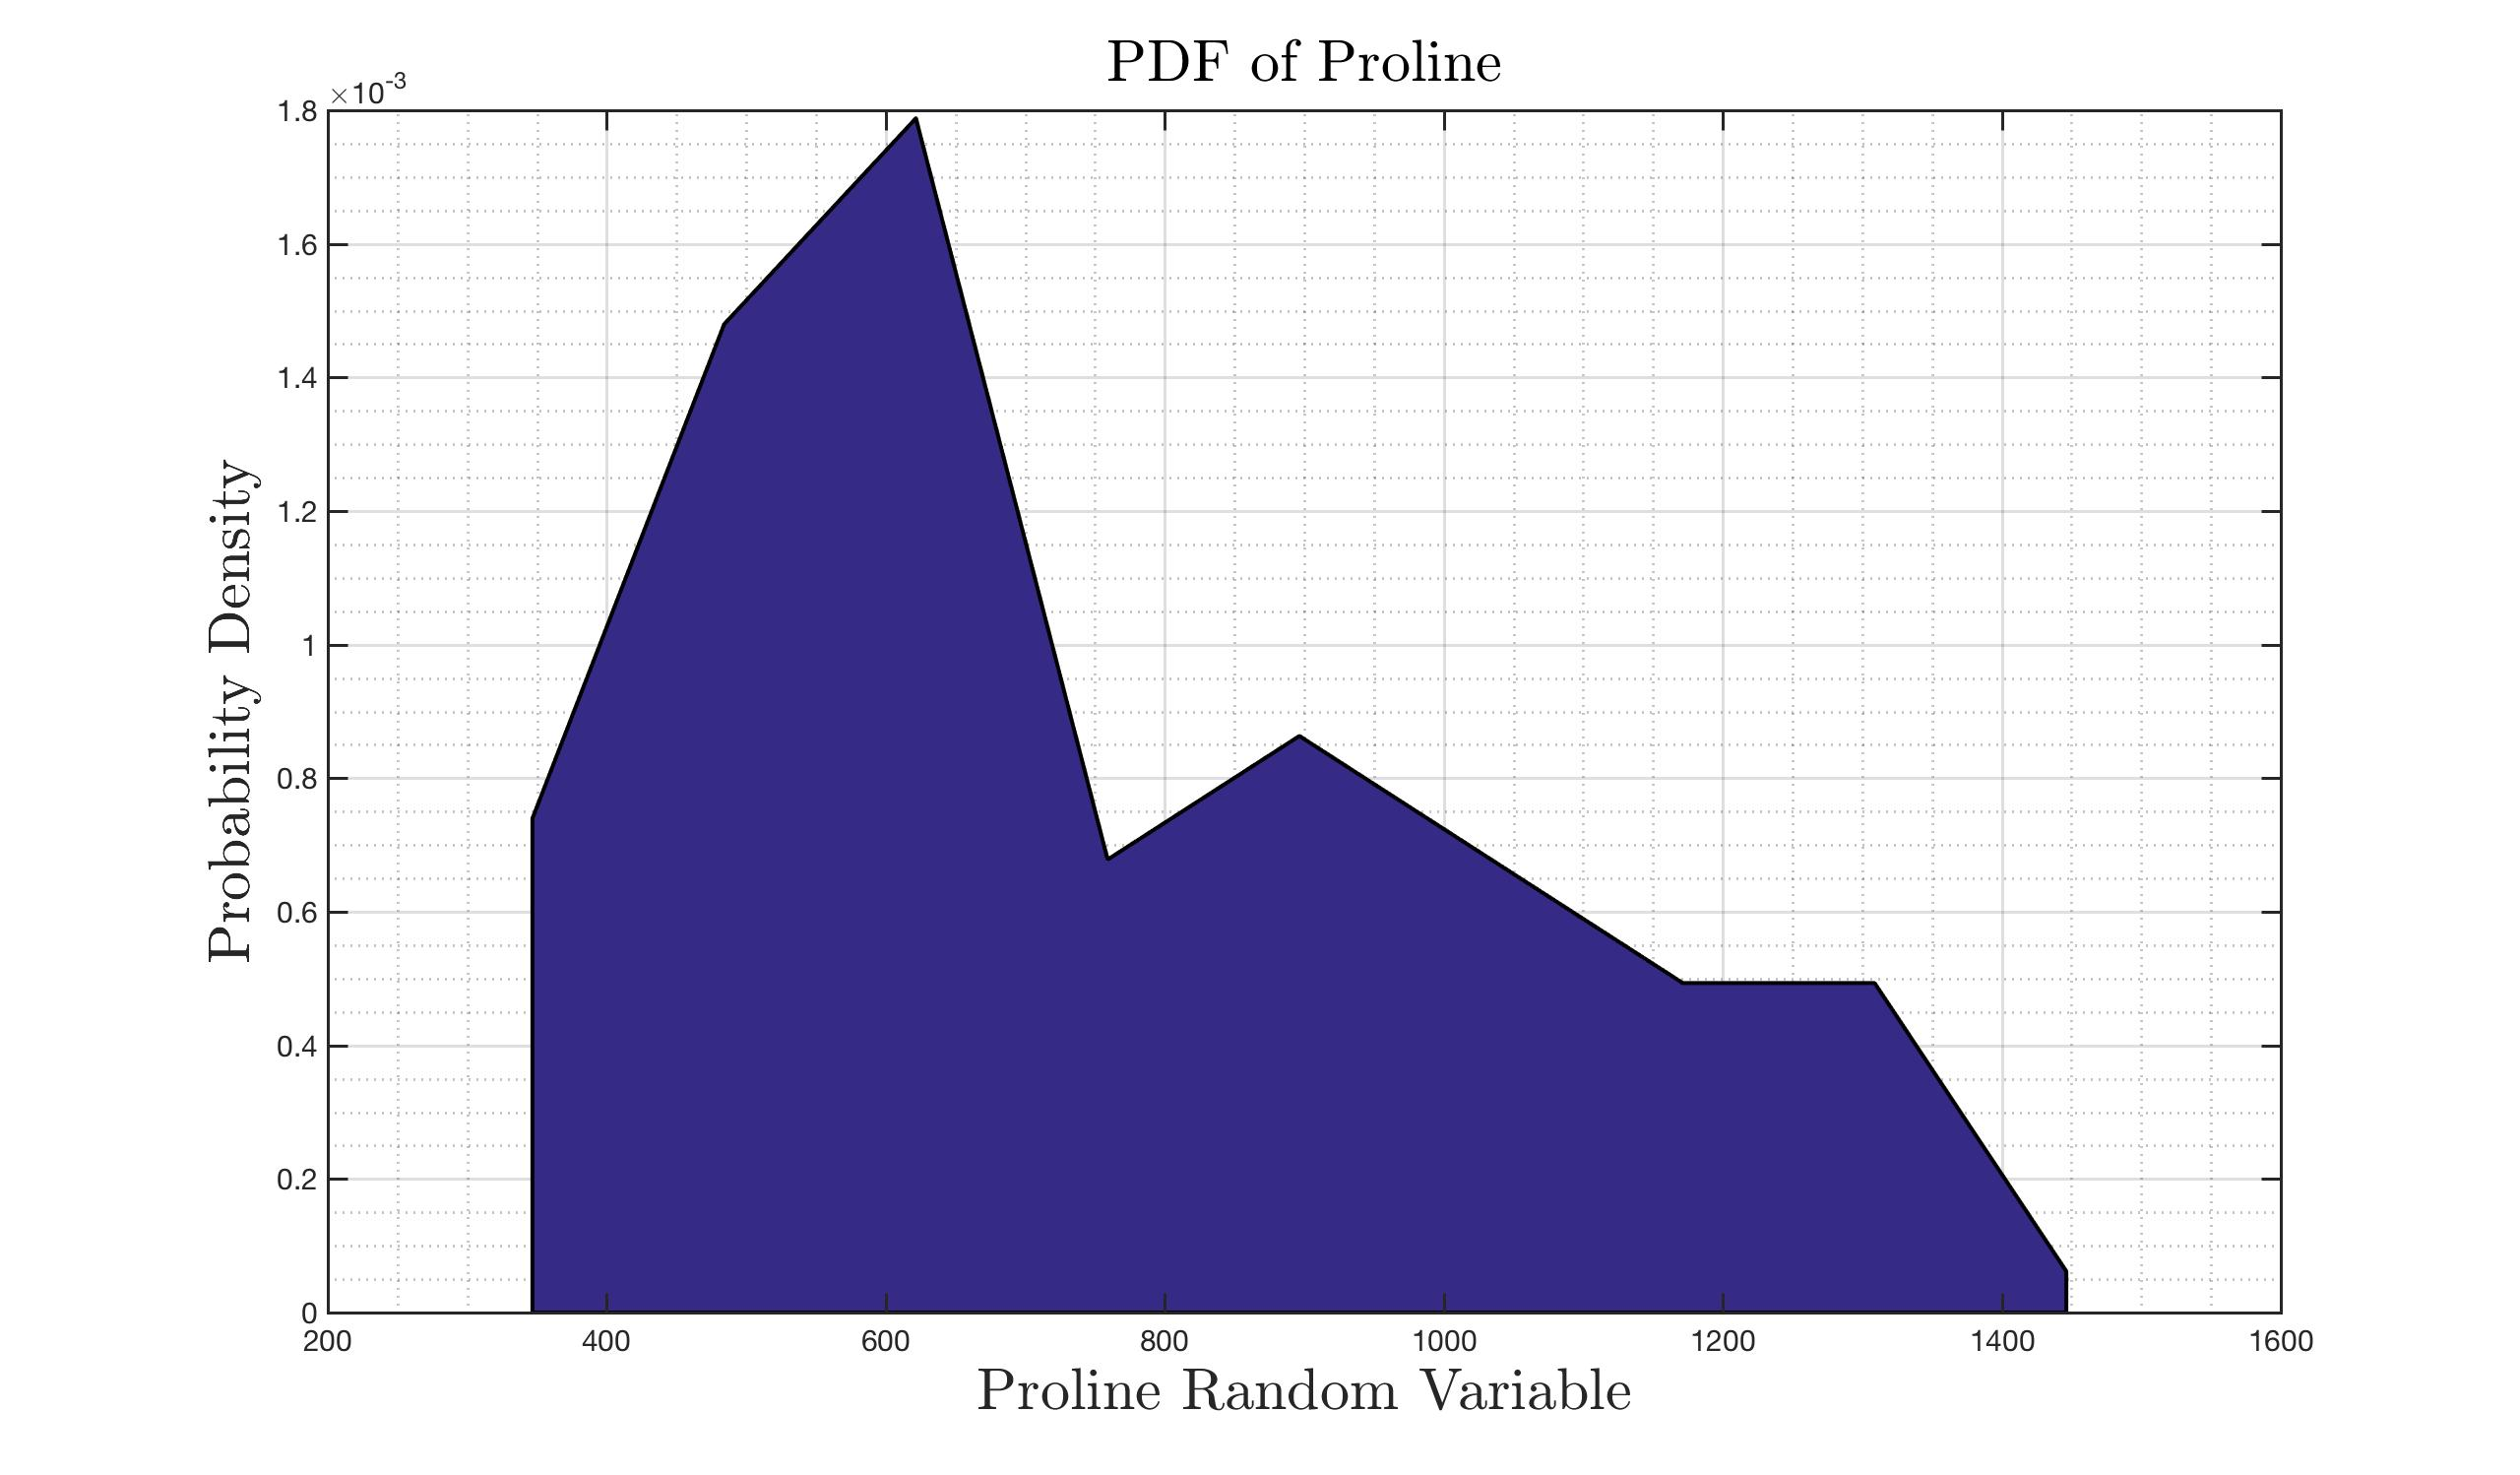
\includegraphics[width=0.4\textwidth]{../results/Q1_ProlineDist}
\caption{Distribution of Proline from all Classes \label{fig:DistProline}}
\end{figure}

\begin{table}[H]
\caption{Sample Means and Standard Dev. for all Training Data \label{tab:statAll}}
\small
\begin{center}
\begin{tabular}{|c| c c c c|}
\hline
\bf Stat/RV & Alcohol & Ash & Hue & Proline \\ [0.5ex]
\hline
\bf Mean & 12.7 & 2.38 & 0.95 & 737 \\ [0.5ex]
\hline
\bf Std. & 0.72 & 0.29 & 0.24 & 287 \\ [0.5ex]
\hline
\end{tabular}
\end{center}
\end{table}

\vspace{-5mm}

Looking at the covariance matrix of the raw training data we can see that proline covaries with all other features quite strongly. This is however due to the fact that proline's distribution has a naturally high variance, thus corrupting the readings. The highest covariance for two different features excluding proline is that of magnesium (feature 5) and colour intensity (feature 10). However, these two features have second and third highest variance distributions. We have to therefore look at the covariance matrix of the normalised feature vectors.

Highest positive covariance is observed for features 6 and 7 (total phenols and flavonoids), whereas the most negative covariance is found for features 2 and 7 (malic acid and flavonoids). The plot of the above cases is shown in Figure \ref{fig:covAll}. This tells us that there is possibly some correlation between the features, e.g. increasing the phenols count increases the number of flavonoids in wine. This does in fact hold in real world, as flavonoids are a subset of natural phenols.

\begin{figure}[H]
\centering
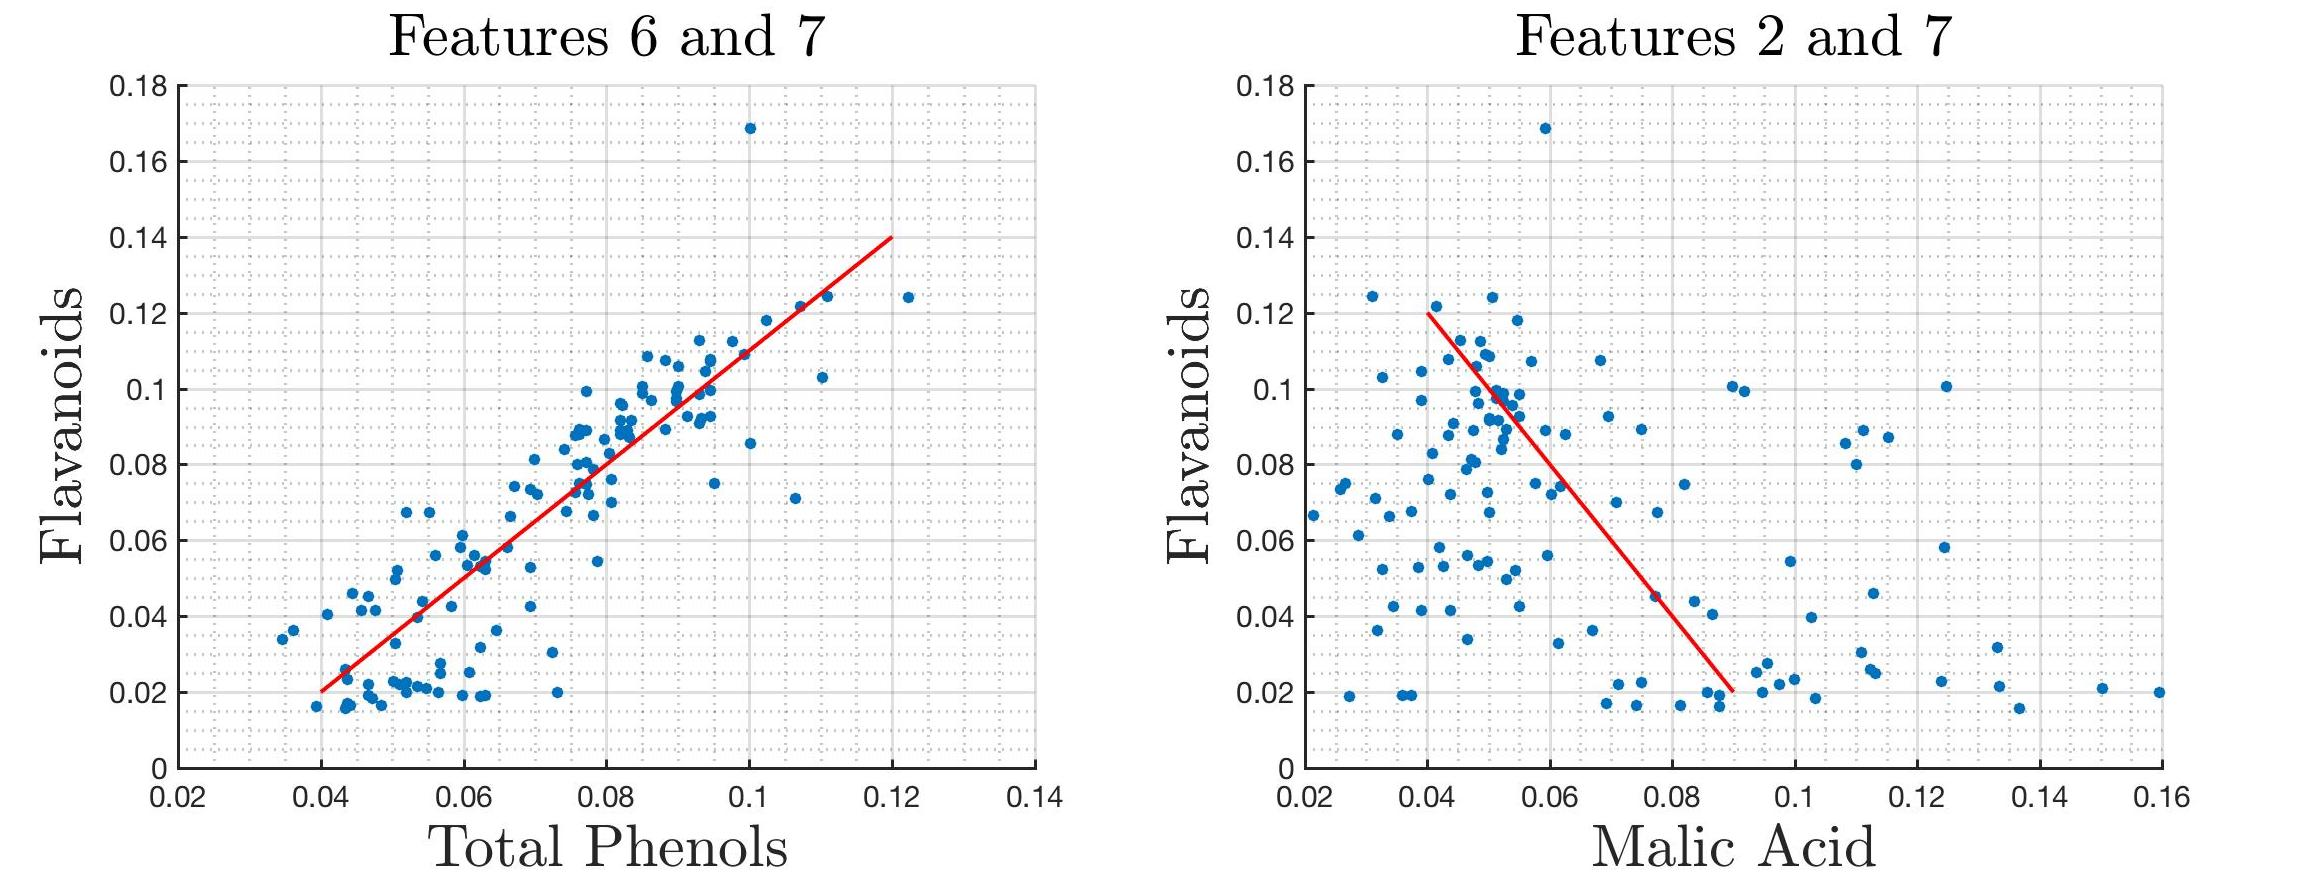
\includegraphics[width=0.5\textwidth]{../results/Q1_covAll}
\caption{Covariance of Features 6 \& 7 and 2 \& 7 Visualised \label{fig:covAll}}
\end{figure}

\vspace{-5mm}

\subsubsection{Individual Classes} \label{sec:CovCla}

\indent \indent As mentioned earlier, the PDF seen in Figure \ref{fig:DistProline} is a summation of three other PDFs for classes 1, 2 and 3. This is shown in Figure \ref{fig:DistProline_Idv}. We can see that in fact, each individual proline random variable can be estimated with a Gaussian distribution. Given that the random variables can be thought of as independent, their sum is also normally distributed.

\begin{figure}[H]
\centering
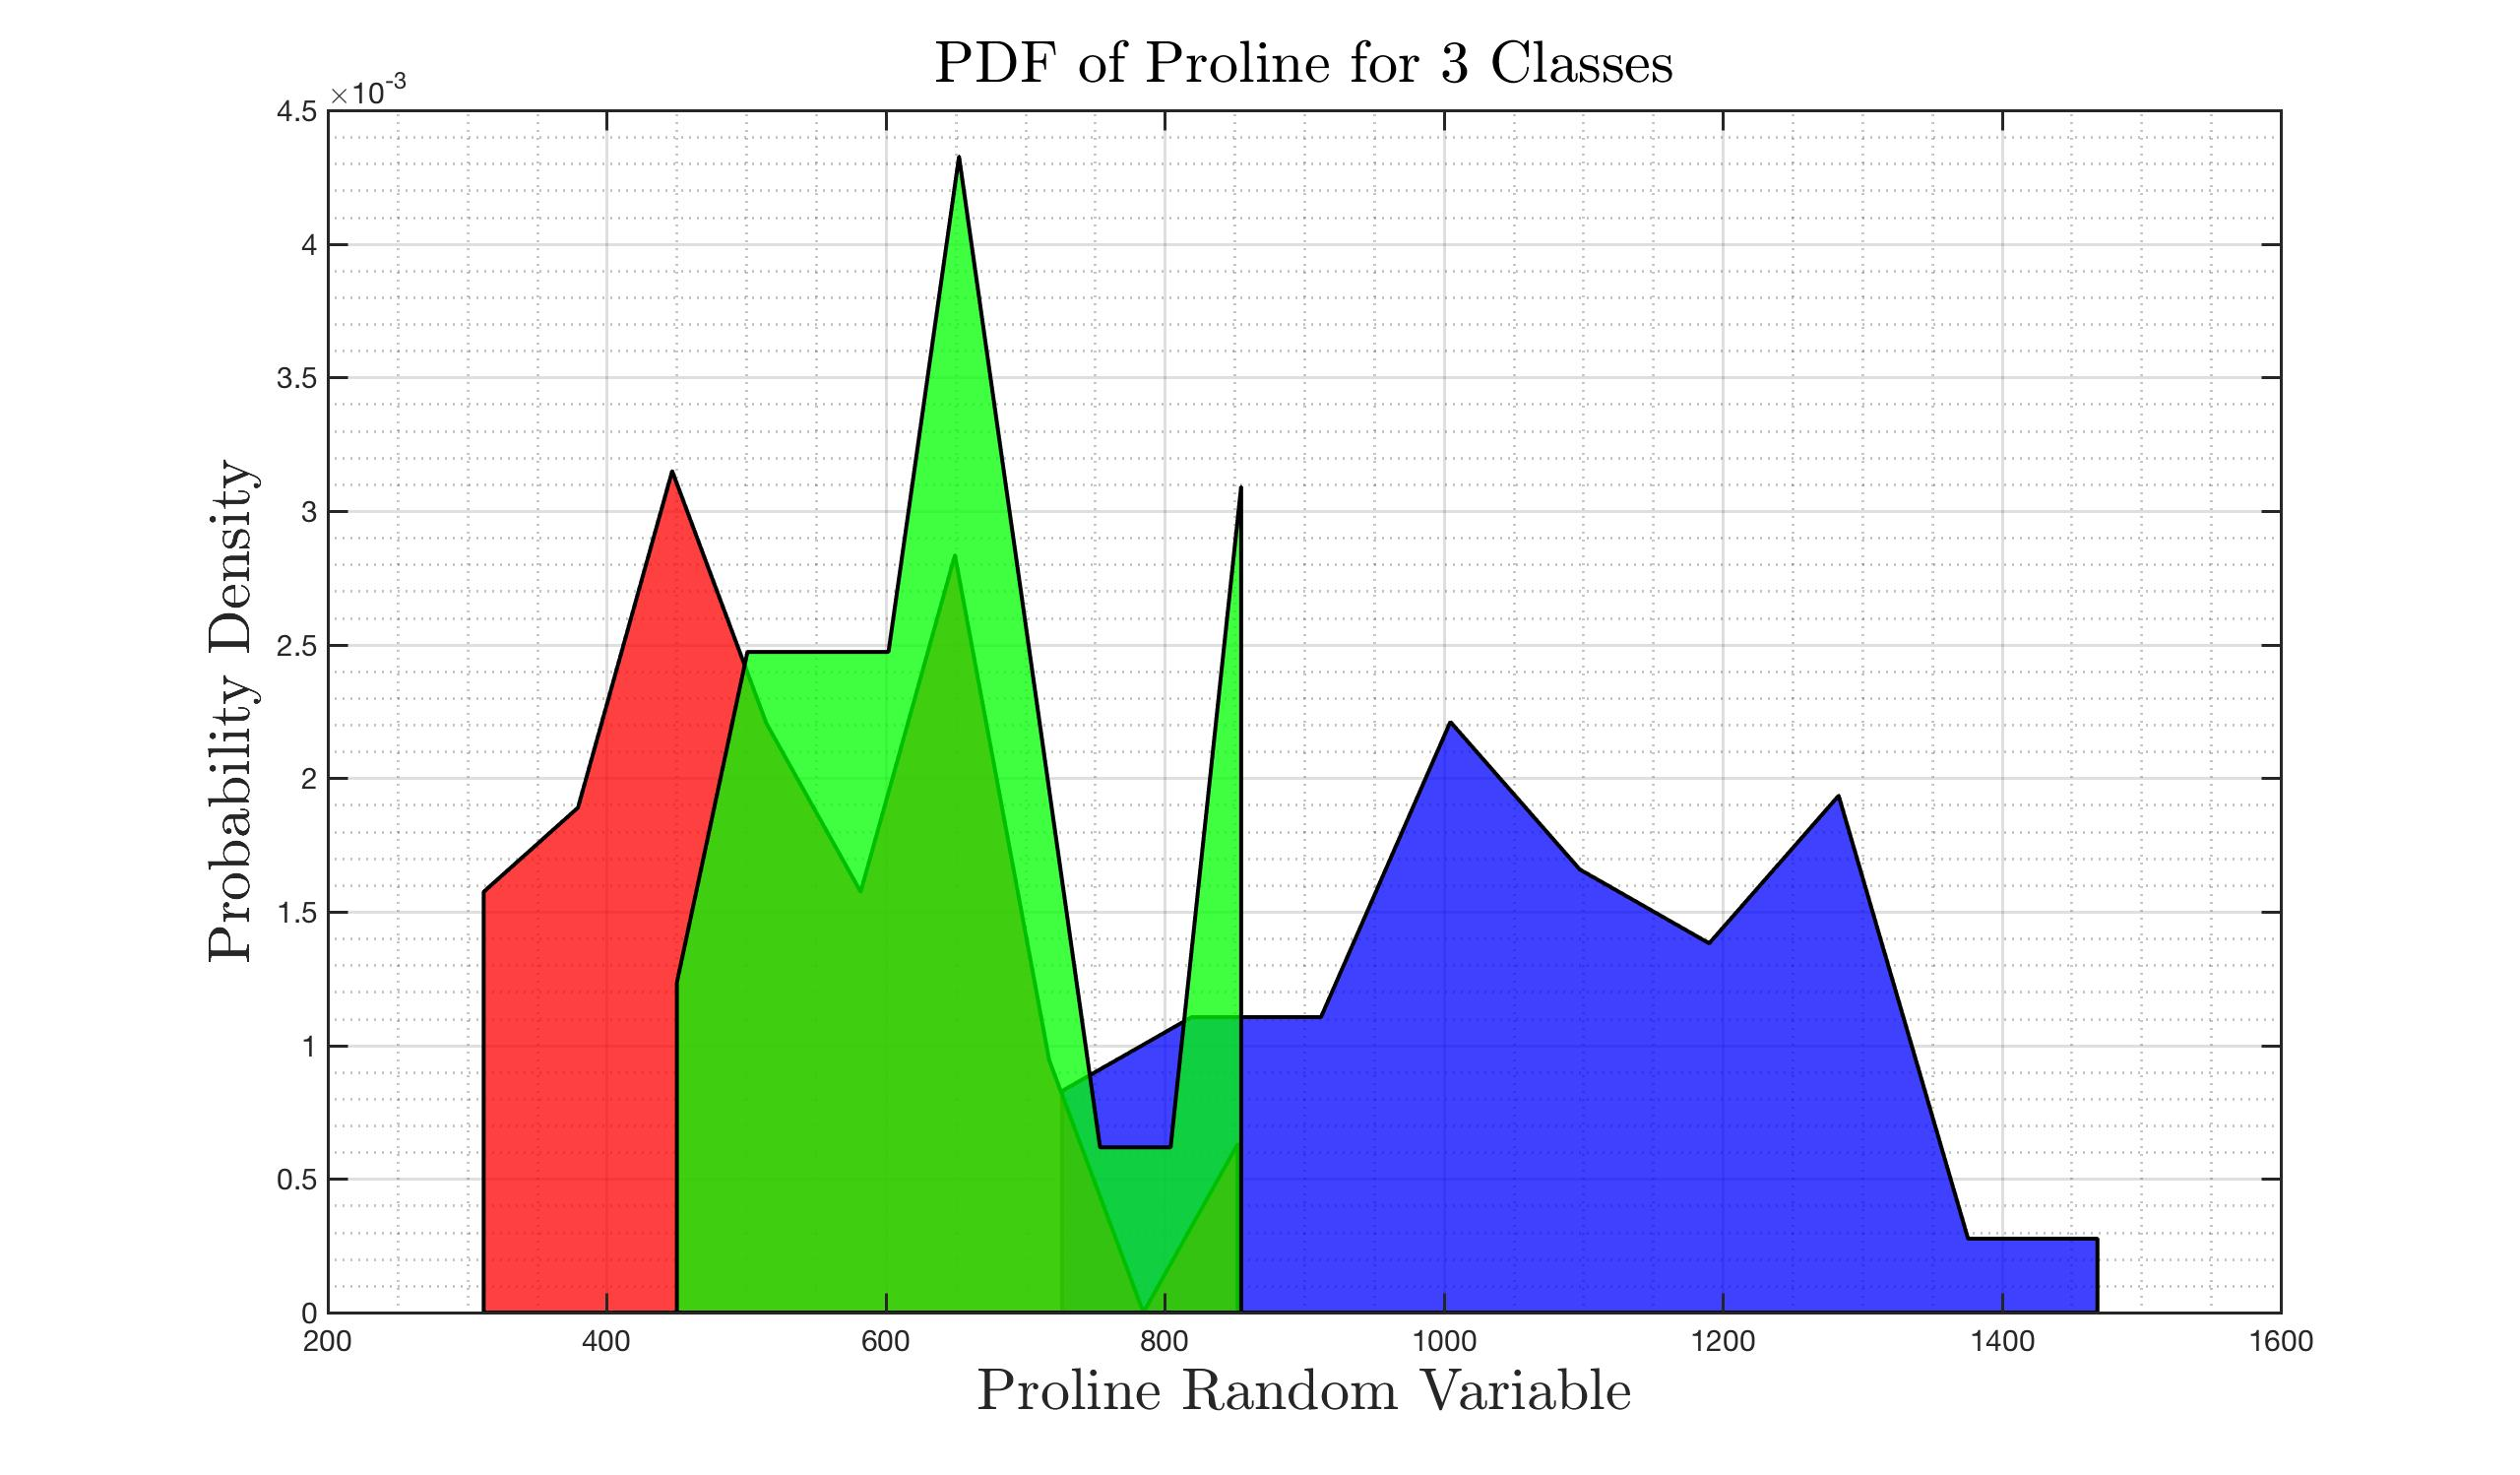
\includegraphics[width=0.4\textwidth]{../results/Q1_ProlineDist_Idv}
\caption{PDF of Proline for Class 1 (blue), 2 (red) and 3 (green) Visualised \label{fig:DistProline_Idv}}
\end{figure}

The above figure shows that each feature in every class can have a very different distribution to other classes and to the overall sum. This is the basis for feature recognition. Given that the features vary from class to class we will be able to determine the test class. For instance in Figure \ref{fig:DistProline_Idv} class 1 clearly stands out. Hence if we test a wine whose proline exceeds 900, it will most definitely belong to class 1. Let us then see how the means and standard deviations of the features in Table \ref{tab:statAll} change when we separate the data.

\begin{table}
\caption{Sample Means and Standard Dev. for each Class \label{tab:statCla}}
\footnotesize
\begin{center}
\begin{tabular}{|c| c c c c|}
\hline
\bf Stat/RV & Alcohol & Ash & Hue & Proline \\ [0.5ex]
\hline
\bf Mean 1 & 13.5 & 2.50 & 1.10 & 1070 \\ [0.5ex]
\hline
\bf Mean 2 & 12.0 & 2.27 & 1.07 & 522 \\ [0.5ex]
\hline
\bf Mean 3 & 12.9 & 2.41 & 0.67 & 647 \\ [0.5ex]
\hline
\bf Std. 1 & 0.31 & 0.26 & 0.12 & 195 \\ [0.5ex]
\hline
\bf Std. 2 & 0.32 & 0.34 & 0.21 & 145 \\ [0.5ex]
\hline
\bf Std. 3 & 0.35 & 0.18 & 0.10 & 121 \\ [0.5ex]
\hline
\end{tabular}
\end{center}
\vspace{-5mm}
\end{table}

Table \ref{tab:statCla} tells us for instance, that wine from class 1 has a higher alcohol contents than the other two classes. Wine from class 3 however is of different colour, meaning it could be a class of white or red wines. Finally, looking at proline concentration, we can see again, that class 1 stands out. A research paper \cite{wine} shows that Sauvignon Blanc and Grillo wines tend to have a much higher proline content than other wines, meaning this can be class of those wines.

 
After dividing the data into classes and calculating their respective covariance matrices we see that those features, which used to have a relatively large covariance, are not necessarily correlated anymore. In Figure \ref{fig:covIdv}, it can be seen that features 2 and 7 for class 3 are completely unrelated.

\begin{figure}[H]
\centering
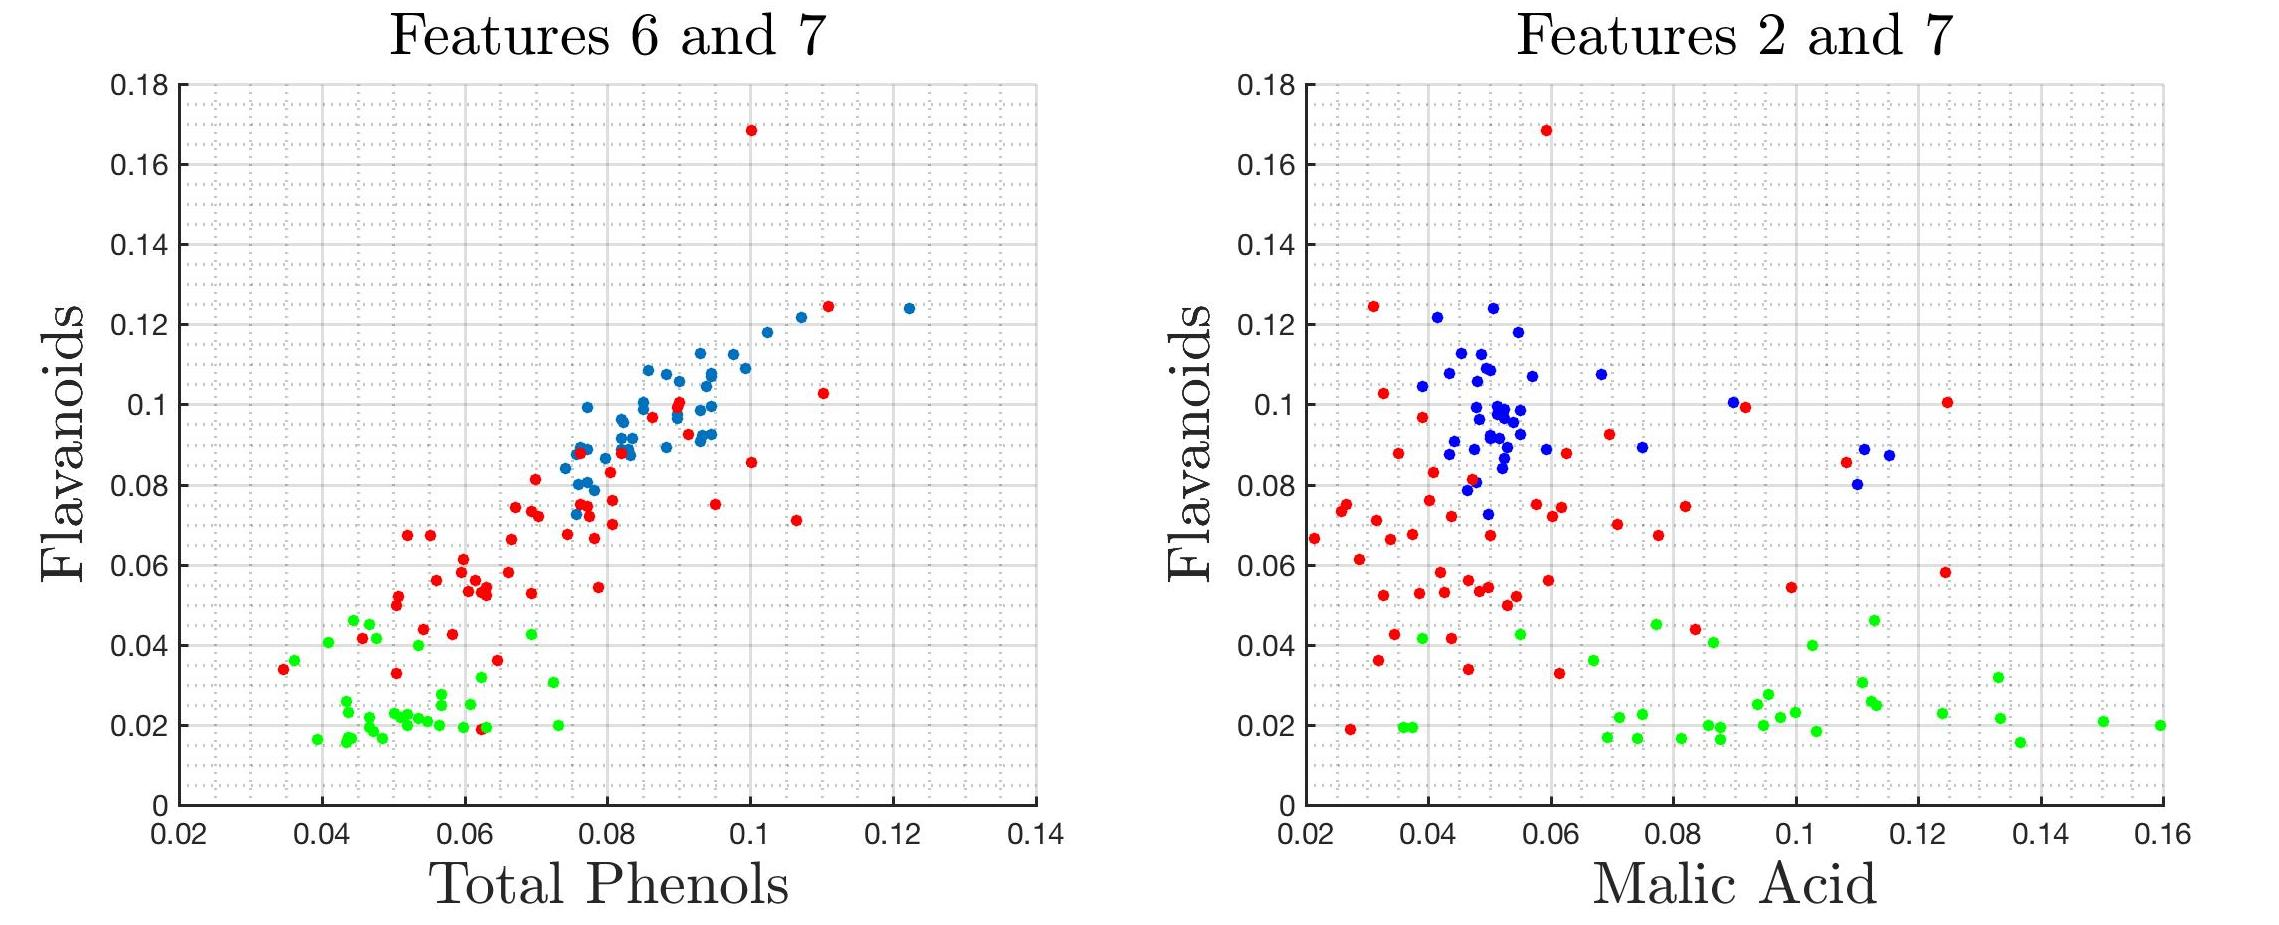
\includegraphics[width=0.5\textwidth]{../results/Q1_covIdv}
\caption{Covariance of Features 6 \& 7 and 2 \& 7  for Class 1 (blue), 2 (red) and 3 (green) Visualised \label{fig:covIdv}}
\end{figure}

\subsection{L1, L2 , Chi-Squared, Histogram Intersection, Correlation Metrics}

In order to assign class to a test wine, we need to employ some similarity measure. The simplest belong to Minkowski's Form - L1 and L2. They measure the Manhattan and Euclidean distances respectively. A more complex approach is to measure the chi-squared distance, which corrects the L2 metric by taking into account the absolute positions of the points in space. Hence if points have relatively large coordinates, the "hit" is allowed to be further away. Similarly, if a point of consideration has relatively small coordinates, then the match must be more precise in order to be classified as a hit. For instance an L1 metric of points $(100,0)$, $(60,0)$ and $(50,0)$, $(10,0)$ would yield 40 for both. However chi-squared distance is 5.05 and 13.7 respectively, meaning even though the two sets of points are equally spaced, the first pair is more likely to be a hit.

In the table below we have summarised the results of the above metric and also histogram intersection and correlation measure. Each metric was used for raw and normalised data.

\begin{table}[H]
\caption{Miss Rates for Various Metrics and Data Form \label{tab:MissMetric}}
\small
\begin{center}
\begin{tabular}{|c| c c c c c|}
\hline
\bf Metric & L1 & L2 & Chi-Sq. &  Hist. & Corr. \\ [0.5ex]
\hline
\bf Miss Raw & 15\% &20\%  & 10\% & 17.5\% & 20\% \\ [0.5ex]
\hline
\bf Miss Norm & 10\% & 12.5\% & 5\% & 25\% & 10\% \\ [0.5ex]
\hline
\end{tabular}
\end{center}
\end{table}

\vspace{-5mm}

The tests employed feature vectors of length 13 each as histograms, with the exception of histogram intersection. In this particular case we have used all of the training data and converted it into 3 histograms - one for each class. Then by transforming each test wine into a histogram with identical bin positions we performed the histogram intersection. We have then varied the number of bins and plotted the resulting accuracy curve. This is shown in Figure \ref{fig:hist}.

\begin{figure}[H]
\centering
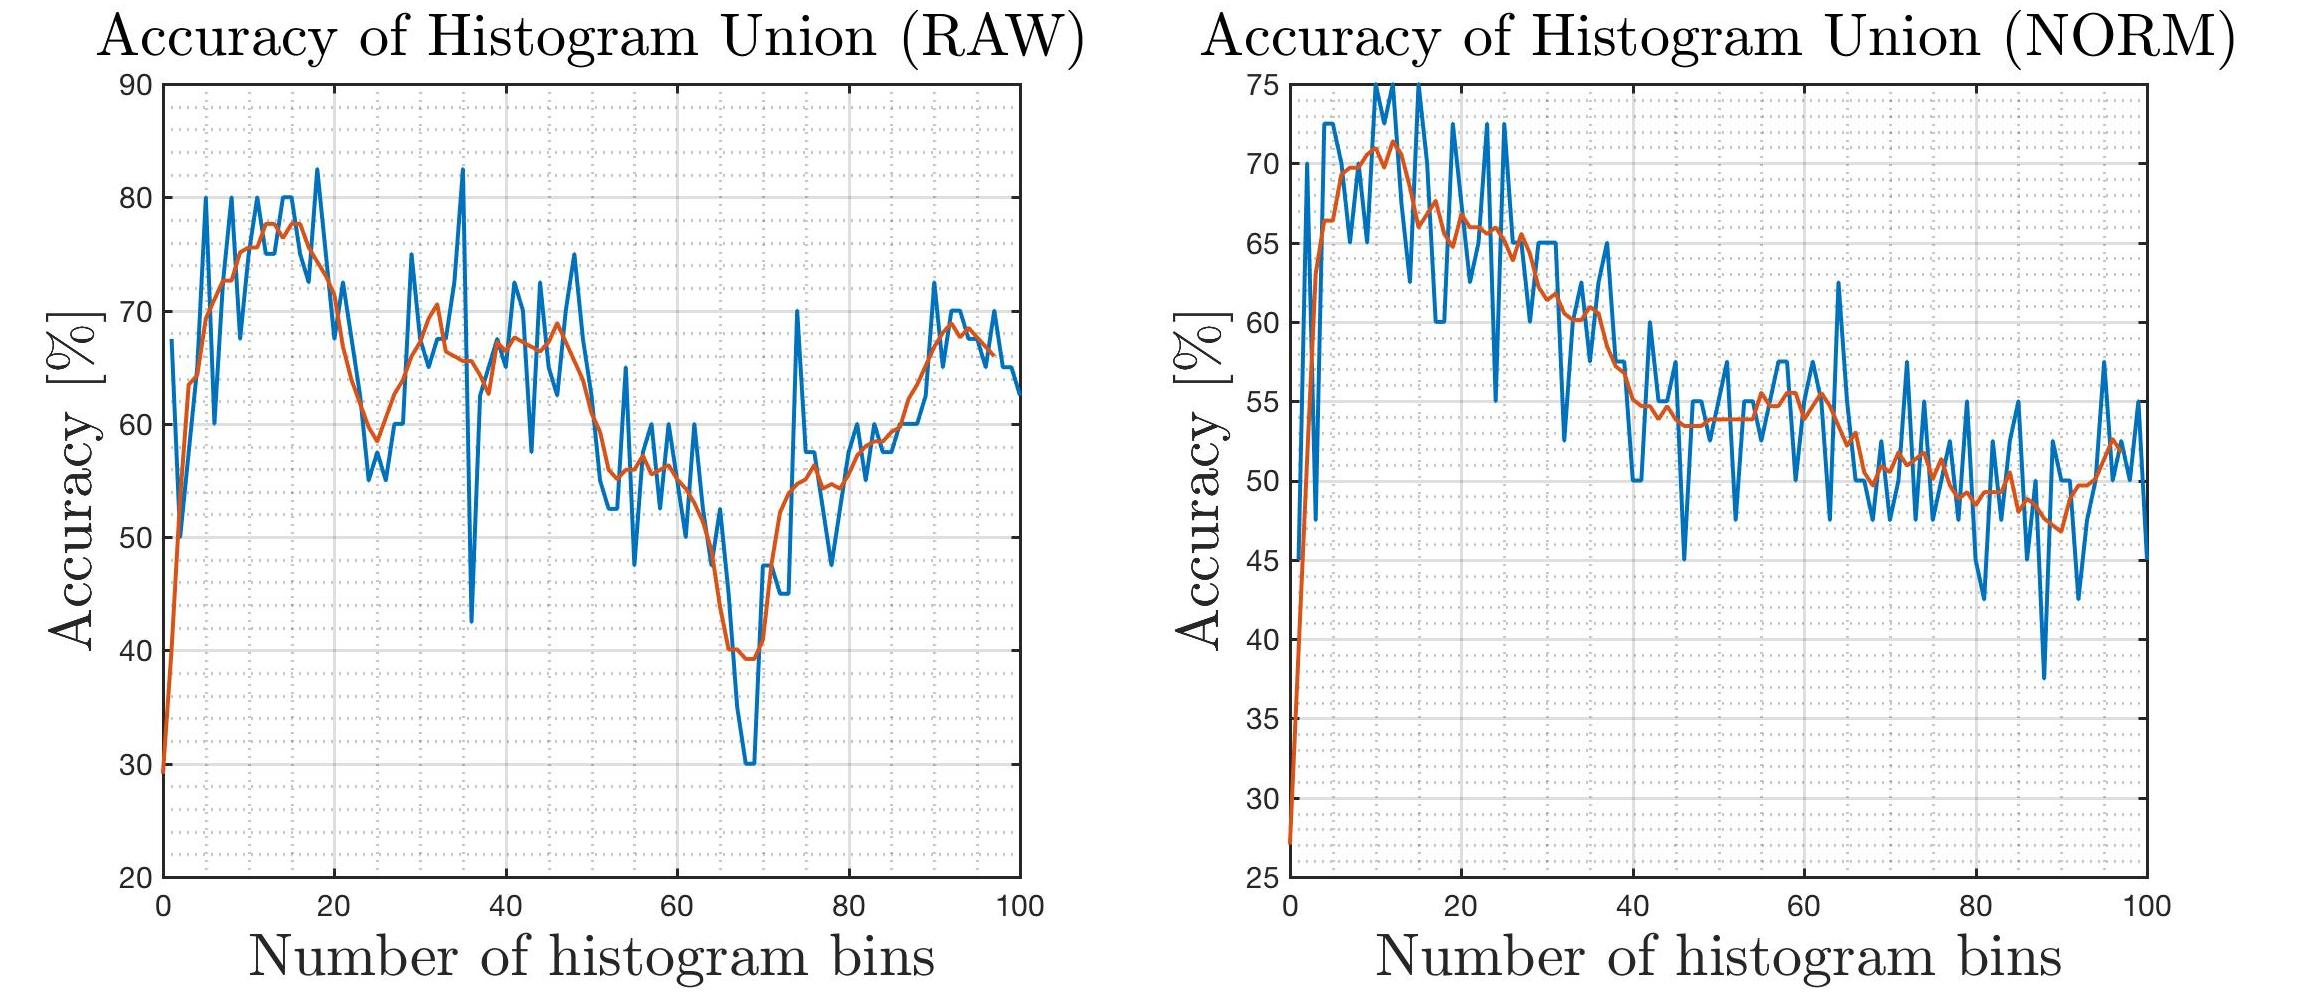
\includegraphics[width=0.5\textwidth]{../results/Q1D_Hist}
\caption{Plots of Hit Rate against Number of Bins for Raw and Normalised Data
\label{fig:hist}}
\end{figure}

Following from Table \ref{tab:MissMetric} it can be deduced that Chi-Squared metric produces best results for both sets of data - raw and normalised. It is however surprising that L1 has produced results more accurate than L2 in either case. It is said \cite{L1L2} that L2 theoretically is superior over L1 as it preserves the distance energy. However, the same source reports that there are practical situations when L1 might be better, such as when there are outliers. L1 is reported to be more robust when the class occupies the space quite sparsely. In this experiment, we have employed the Nearest Neighbour method. Hence the class spread is unimportant. Thus the superiority of L1 over L2 possibly comes from this particular set of training and testing data.

Comparatively L1, L2 and Cross Correlation metrics are very similar, each producing incorrect classifications 10 to 20\% of the time. Cross Correlation defined as a square of the Euclidean distance, is supposed to be more robust to outliers as well. The results should not vary greatly from the L2 metric as they are related by a square root. 

There is a general trend that metrics produce better results when the data is normalised. This is with exception of Histogram Intersection, as seen in Figure \ref{fig:hist}. The accuracy of that metric varies with number of bins. In both cases, the graphs peak at around 13 to 15 bins, which agrees with the feature size - 13. For normalised data, the trend after the peak is non-increasing. For raw data, on the other hand, the trend varies, with its local minimum at around 68 bins. 

\subsection{Mahalanobis Distance Metric}

The Mahalanobis Distance Metric is similar to the L2 metric, except that a linear transformation is performed on the testing and training data before taking the measurement. This linear transformation, performed using the training data's covariance matrix, projects the data onto a linear subspace. A new set of axes is used, reshaping the data. The direction of the first axis is the direction of the greatest variance of the data, and the second axis is perpendicular to the first axis in the direction of the greatest variance, and so on for however many features the data has. The transformation also normalises the data, so that the units of each axis are the standard deviation along it. 

By taking the Euclidean distance of projections onto this subspace, a metric is created that accounts for the fact that variances are different for each feature, accounts for the covariances between features, and reduces to a standard Euclidean distance for uncorrelated features with unit variance.

The Mahalanobis distance between two points was calculated as $d_S(x_1,x_2) = ||\mathbf{G}x_1 - \mathbf{G}x_2||^2_2$, where $x_1$ is the testing point, $x_2$ is the training point, $\mathbf{S}$ is the covariance matrix of the training data, $\mathbf{G}$ is the Cholesky decomposition of $\mathbf{S}^{-1}$, and $||x||^2_2$ is the squared L2 norm of $x$.

This metric was tested in two ways. Firstly, the Mahalanobis distance was measured using the covariance matrix of all the training data. Secondly, the Mahalanobis distance was measured with separate covariance matrices for each class in the training data. The miss rates are shown in Table \ref{tab:MissMahal}. 

\begin{table}[H]
\caption{Miss Rates for Mahal tests \label{tab:MissMahal}}
\footnotesize
\begin{center}
\begin{tabular}{|c| c c|}
\hline
\bf Covaraince Matrix & Single & Separated \\ [0.5ex]
\hline
\bf Miss Rate & 20\% & 0\% \\ [0.5ex]
\hline
\end{tabular}
\end{center}
\end{table}

It can be seen that the single covariance matrix method has 80\% success, whereas the separated covariance matrices method are 100\% successful. These results are explored further in Figure \ref{fig:Mahal}.

\begin{figure}
\centering
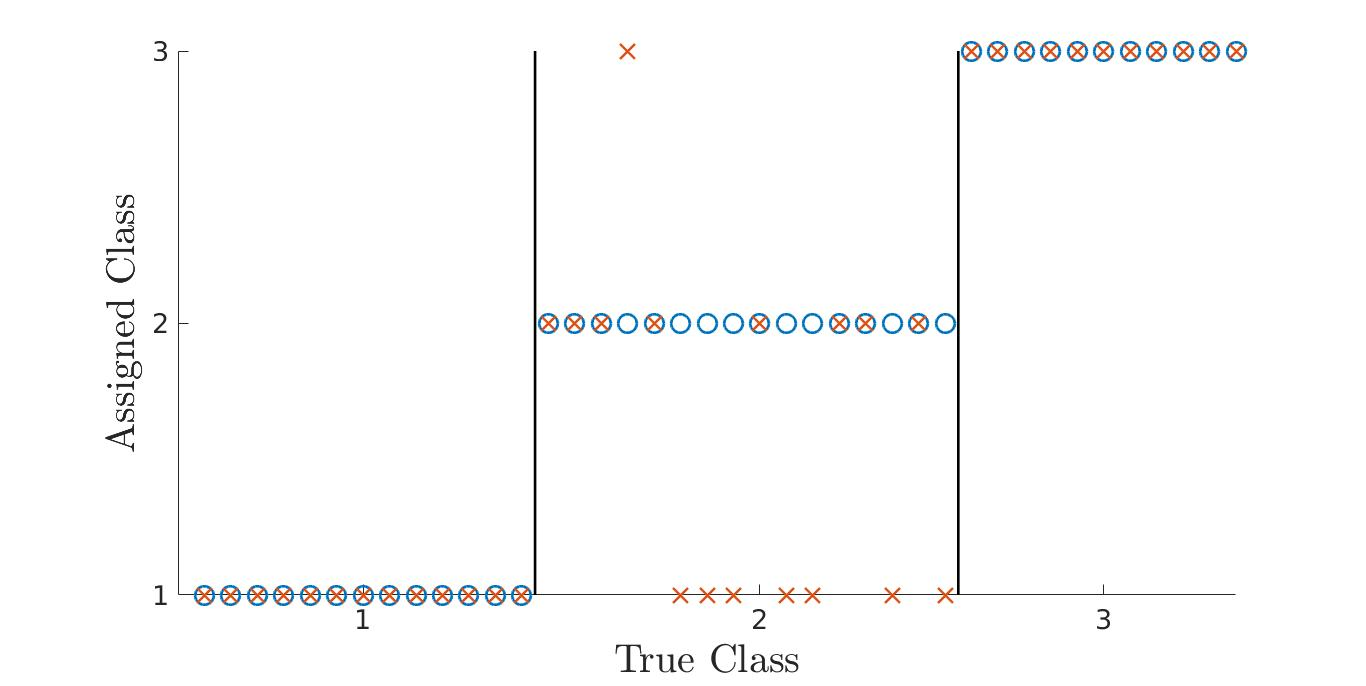
\includegraphics[width=0.5\textwidth]{../results/Q1Db_Success}
\caption{Classification results for Mahalanobis distance metric. Blue circles - Separated covariance matrices, Red crosses - Single covariance matrix
\label{fig:Mahal}}
\end{figure}

It can be seen that both tests were fully successful for classes 1 and 3, but for class 2, the method with the single covariance matrix had several failures. Seven data points from class 2 were assigned to class 1, and one more was assigned to class 3, which suggests that class 2 is too close to the other classes for it to be clearly distinguished from the others. However, for the separated covariance matrices, the classes were individually projected in to a subpspace that enhanced their classification, so the classes could be more easily distinguished, leading to a 100\% success rate.

%\vspace{-6mm}

\section{K-means Clustering}
\subsection{k = 3 Clusters}
In order to implement k-means clustering Matlab functions {\tt\small kmeans} and {\tt\small knnsearch} were used. The first test for $k=3$ involved normalised training and testing data. For clustering the following metrics were used: L1, L2, cosine and cross correlation.
For classification the following metrics were used: L1, L2, Cross Correlation, Chi-Squared, Histogram Intersection, and Mahalanobis Distane. The accuracy results (hit rate) are reported in Table \ref{tab:kmeans3}.

Note that {\tt\small kmeans} function does not produce the same results every time, since the algorithm begins by placing the centres at arbitrary points in space. Hence they converge to different location most of the time. Thus in order to assess the performance each combination of kmeans and kNN algorithms was run 1000 times and average result has been calculated. Additionally we have included Table \ref{tab:kmeans_3max} showing best case performance, when clustering has been particularly successful, showing what can ideally be achieved.

\begin{table}[H]
\caption{Mean Accuracy of k-means Clustering and kNN Classification over 1000 Trials \label{tab:kmeans3}}
\footnotesize
\begin{center}
\begin{tabular}{|c| c c c c|}
\cline{2-5}
\multicolumn{1}{c|}{ } & \multicolumn{4}{|c|}{\bf Kmeans Clustering, k = 3} \\
\hline

\bf kNN &\bf L1 &\bf L2 &\bf Cosine &\bf Corr \\ [0.5ex]
\hline
\bf L1 & 84.08\% & 67.39\%  & 27.50\% & 43.49\%\\ [0.5ex]
\hline
\bf L2 & 87.78\% & 68.83\%  & 84.14\% & 69.41\%\\ [0.5ex]
\hline
\bf Corr. & 81.53\% & 66.27\%  & 82.00\% & 84.83\%\\ [0.5ex]
\hline
\bf Chi-Sq & 86.47\% & 68.80\%  & 69.42\% & 17.25\%\\ [0.5ex]
\hline
\bf Hist. & 62.25\% & 53.27\%  & 37.89\% & 43.49\%\\ [0.5ex]
\hline
\bf Mahal. & 85.79\% & 71.13\% & 32.87\% & 42.51\% \\ [0.5ex]
\hline
\end{tabular}
\end{center}
\end{table}

\begin{table}
\caption{Max Accuracy of k-means (3) Clustering and kNN Classification over 1000 Trials \label{tab:kmeans_3max}}
\footnotesize
\begin{center}
\begin{tabular}{|c| c c c c|}
\cline{2-5}
\multicolumn{1}{c|}{ } & \multicolumn{4}{|c|}{\bf Kmeans Clustering, k = 3} \\
\hline
\bf kNN &\bf L1 &\bf L2 &\bf Cosine &\bf Corr \\ [0.5ex]
\hline
\bf L1 & 85.00\% & 87.50\%  & 27.50\% & 60.00\%\\ [0.5ex]
\hline
\bf L2 & 90.00\% & 87.50\%  & 92.50\% & 95.00\%\\ [0.5ex]
\hline
\bf Corr. & 82.50\% & 85.00\%  & 85.00\% & 87.50\%\\ [0.5ex]
\hline
\bf Chi-Sq & 87.50\% & 87.50\%  & 75.00\% & 30.00\%\\ [0.5ex]
\hline
\bf Hist. & 75.00\% & 65.00\%  & 50.00\% & 72.50\%\\ [0.5ex]
\hline
\bf Mahal. & 90\% & 92.50\% & 40.00\% & 65.00\%\\ [0.5ex]
\hline
\end{tabular}
\end{center}
\end{table}

An example of kmeans clustering is shown in Figure \ref{fig:clusFig}. In this example \textit{cityblock} or Minkowski form distance with $p=1$ was used. It can be seen comparing left and right images that that some point were assigned to the wrong class.

\begin{figure}
\centering
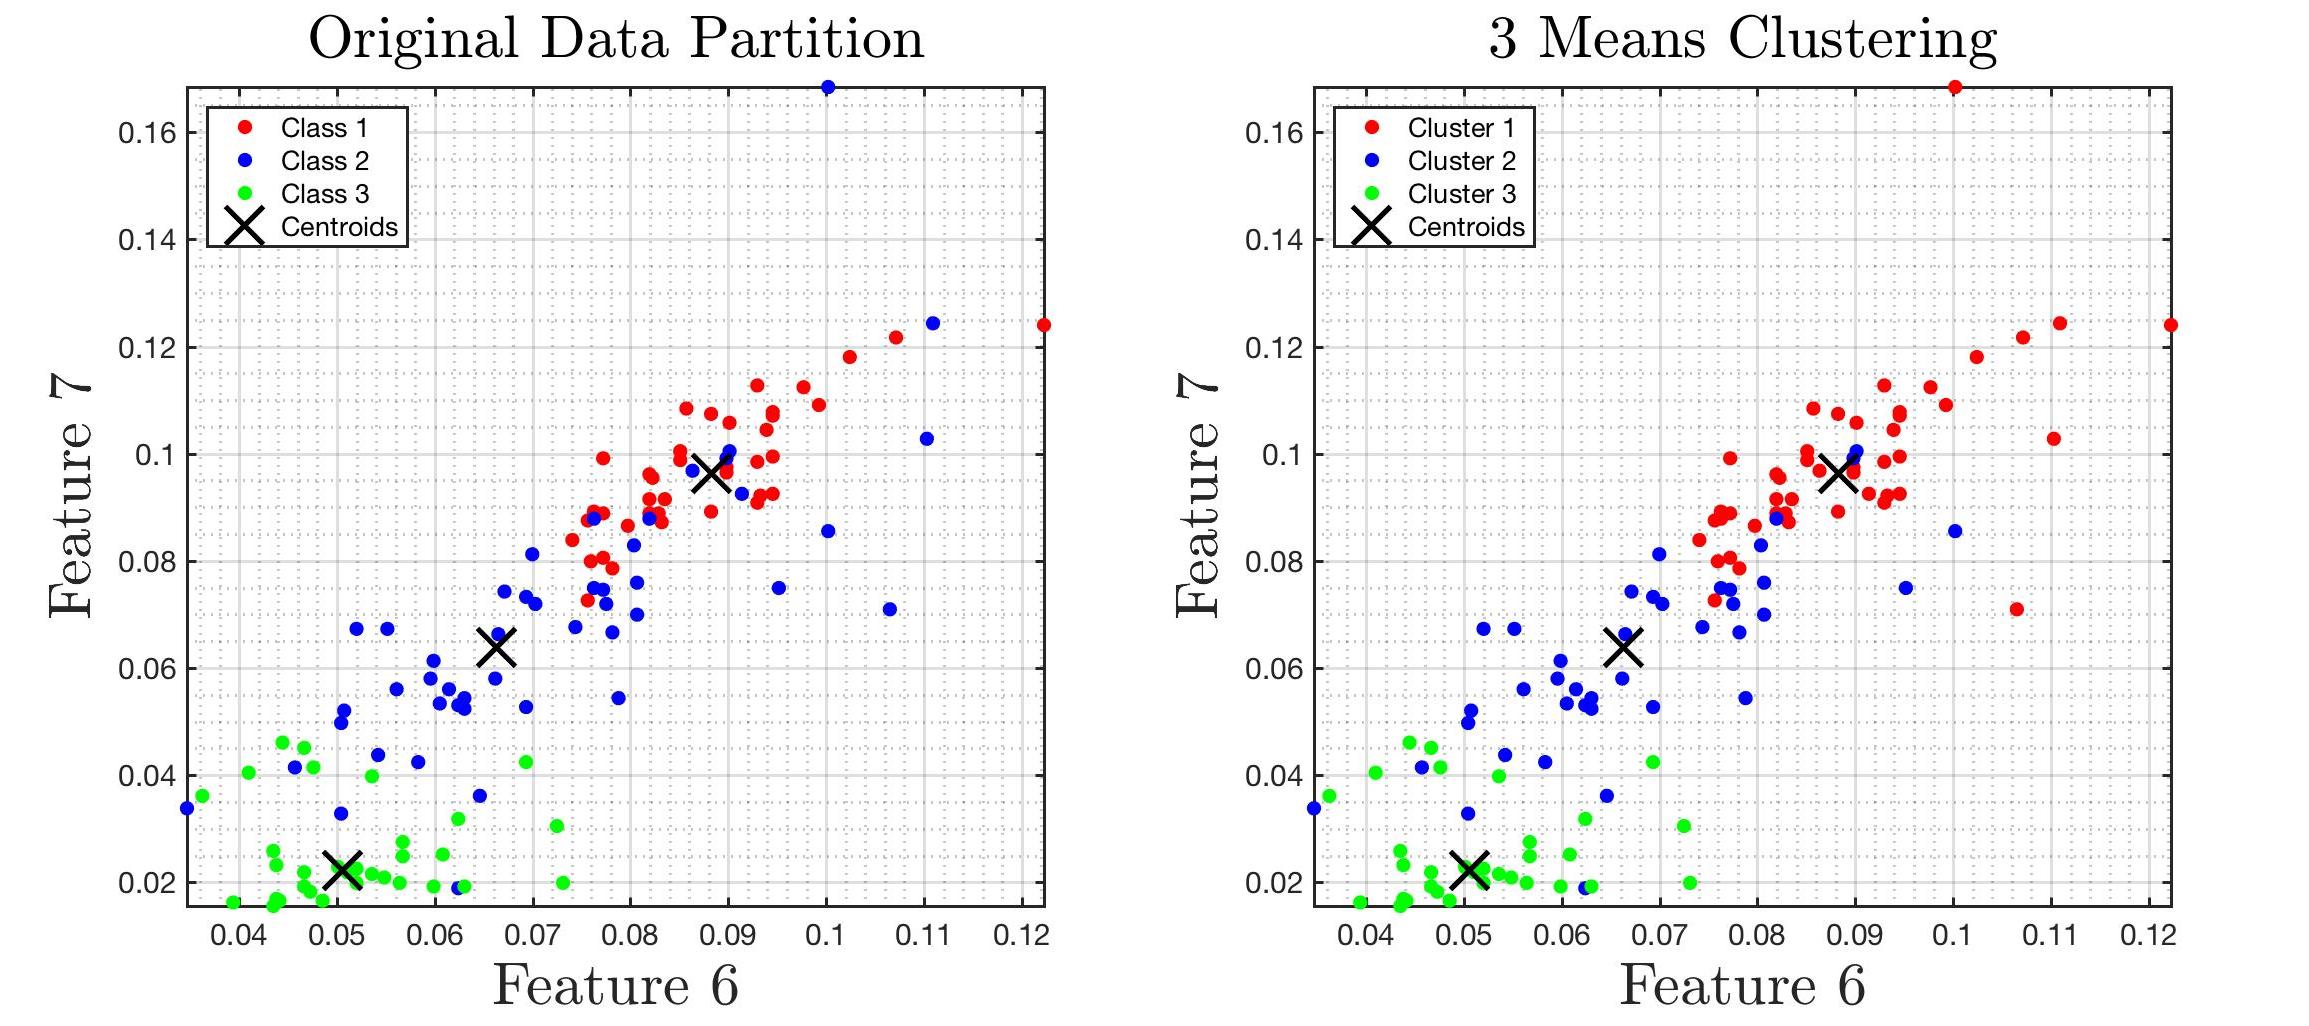
\includegraphics[width=0.5\textwidth]{../results/kmeans_part}
\caption{Comparison of Original Data (left) and kmeans Partitioned Data (right)
\label{fig:clusFig}}
\end{figure}
 
Overall, \textit{L1} clustering is producing the best results with every Nearest Neighbour methods. The best performance is found when using \textit{L1} to cluster the training data and \textit{L2} to classify testing data - averaging 87.78\% success rate.

It should be expected that combinations of the same algorithm to cluster and classify should be producing quite high results as well. This is clearly seen for \textit{L1} and \textit{Correlation}, where the hit rates both exceed 84\%.

In absolute terms, the best performance has been observed for data clustered using \textit{cosine} and classified using \textit{L2} - peaking at 95\%. On the other hand the worst combination both on average and in absolute terms has been found to be \textit{Correlation} for clustering and \textit{Chi-Square} for classification - 17.25\% and 30.0\% respectively.
 
The Mahalanobis distance test from the previous section with a single covariance matrix achieved 80\% accuracy, so most of the methods that used \textit{L1} clustering surpassed it, but most of the methods with other clustering techniques did not beat it. Within \textit{L1}, only the \textit{Histogram Intersection} classification had a maximum that was below 80\%. The Mahalanobis test with separated covariance matrices was 100\%, so none of the k means 3 techniques were able to match it, including the techniques that used \textit{Mahalanobis Distance} for classification.
 
\subsection{k = 10 Clusters}

The experiment has been repeated for 10 clusters, which exceeds number of classes. How this will affec the results isn't obvious. For more clusters, the grain size becomes smaller and thus training data is divided more accurately. For instance if we took the most extreme case, where cluster size becomes 1 - each cluster will be assigned the class of its only member, thus reaching 100\% accuracy. However, as we decrease the cluster size the problem becomes more and more like a simple one-to-one kNN, which, as shown in sections before can produce much worse results. \footnote{This is true when considering absolute maxima for each method shown in Table \ref{tab:kmeans_3max}}

The mean and maximum data is shown in Tables \ref{tab:kmeans10}
and \ref{tab:kmeans_max10}. Comparing the results from Tables \ref{tab:kmeans3} and \ref{tab:kmeans10} on one to one basis we see that in most cases the performance has increased. A slight drop in accuracy is observed for those metrics that were already over 80\% accurate. 

Most notable performance increases have been observed for clustering using \textit{L2}. For $k=3$ \textit{L2} has been producing results of around 65\%, whereas for $k=10$ this has increased to 85\%. Finally, looking at absolute maxima, $k=10$ has reached 100\% hit rate, when employing \textit{Correlation} for clustering and classification, \textit{L1} and \textit{L2} for clustering and \textit{Chi-Squared} for classification, and \textit{L1} for clustering and Mahalanobis for classification.

At 80\% success, the Mahalanobis distance with a covariance matrix from all the training data is lower than the \textit{L1} and \textit{L2} clustering techniques, with the exception of the \textit{Histogram Intersection} classifier. The \textit{Correlation} classifier has a higher mean accuracy than the Mahalanobis distance for the \textit{Cosine} and \textit{Correlation} clustering methods as well.


\begin{table}[H]
\caption{Mean Accuracy of k-means (10) Clustering and kNN Classification over 1000 Trials \label{tab:kmeans10}}
\footnotesize
\begin{center}
\begin{tabular}{|c| c c c c|}
\cline{2-5}
\multicolumn{1}{c|}{ } & \multicolumn{4}{|c|}{\bf Kmeans Clustering, k = 10} \\
\hline

\bf kNN &\bf L1 &\bf L2 &\bf Cosine &\bf Corr \\ [0.5ex]
\hline
\bf L1 & 88.07\% & 87.09\%  & 32.59\% & 51.26\%\\ [0.5ex]
\hline
\bf L2 & 87.19\% & 85.98\%  & 82.36\% & 62.10\%\\ [0.5ex]
\hline
\bf Corr. & 85.85\% & 84.13\%  & 85.50\% & 85.61\%\\ [0.5ex]
\hline
\bf Chi-Sq & 88.18\% & 87.02\%  & 64.11\% & 30.48\%\\ [0.5ex]
\hline
\bf Hist. & 65.45\% & 70.12\%  & 38.44\% & 51.26\%\\ [0.5ex]
\hline
\bf Mahal. & 82.36\% & 83.76\% & 34.45\% & 28.10\%\\ [0.5ex]
\hline
\end{tabular}
\end{center}
\end{table}

\begin{table}[H]
\caption{Max Accuracy of k-means (10) Clustering and kNN Classification over 1000 Trials \label{tab:kmeans_max10}}
\footnotesize
\begin{center}
\begin{tabular}{|c| c c c c|}
\cline{2-5}
\multicolumn{1}{c|}{ } & \multicolumn{4}{|c|}{\bf Kmeans Clustering, k = 10} \\
\hline

\bf kNN &\bf L1 &\bf L2 &\bf Cosine &\bf Corr \\ [0.5ex]
\hline
\bf L1 & 97.50\% & 97.50\%  & 47.50\% & 90.00\%\\ [0.5ex]
\hline
\bf L2 & 97.50\% & 97.50\%  & 95.00\% & 95.00\%\\ [0.5ex]
\hline
\bf Corr. & 97.50\% & 95.00\%  & 97.50\% & 100.00\%\\ [0.5ex]
\hline
\bf Chi-Sq & 100.00\% & 100.00\%  & 90.00\% & 57.50\%\\ [0.5ex]
\hline
\bf Hist. & 85.00\% & 90.00\%  & 62.50\% & 90.00\%\\ [0.5ex]
\hline
\bf Mahal. & 100.00\% & 97.50\% & 52.50\% & 62.50\%\\ [0.5ex]
\hline
\end{tabular}
\end{center}
\end{table}

The Mahalanobis distance with separated covariance matrices has 100\% success, so is only matched by the maximum accuracies for the \textit{L1} and \textit{L2} clustering techniques with \textit{Chi-Squared} classification, \textit{L1} clustering with the \textit{Mahalanobis} classifier, and \textit{Correlation} for both clustering and classification.

\section{Neural Network}

To train the Neural Networks with the wine data provided we have used the raw as opposed to the normalised feature vectors. Instruction from lectures and Matlab documentation \cite{MatlabWine} were considered.  Finally, we have ensured that we use all of the training data to train the neural networks by inserting the following lines of code:

\begin{center}
\minibox[frame]{
net.divideParam.trainRatio = 100/100 \\     
net.divideParam.valRatio = 0/100 \\     
net.divideParam.testRatio = 0/100 \\
} 
\end{center}


\subsection{Hidden Layer Size}
The best starting point for a hidden layer size is double the input layer size \cite{NN_Java}. Based on the outcome of that, the hidden layer size should then be varied accordingly. In this experiment, the hidden layer size was varied from 1 to 30 in order to estimate the optimal size. For the duration of this test, the neural network had the following structure.

\begin{center}
\framebox[1.3\width]{\tiny \bf INPUT LAYER (13)} \\

\centering
$\downarrow$ \\

\centering
\framebox[1.3\width]{\tiny \bf SINGLE HIDDEN LAYER (1 TO 30)}\\

\centering
$\downarrow$\\

\centering
\framebox[1.3\width]{\tiny \bf OUTPUT LAYER (3)}\\

\end{center}

Having run the network for all of the above hidden layer sizes thirty times, the mean accuracy for each layer size has been plotted (Figure \ref{fig:HidSiz}).

\begin{figure}[H]
\centering
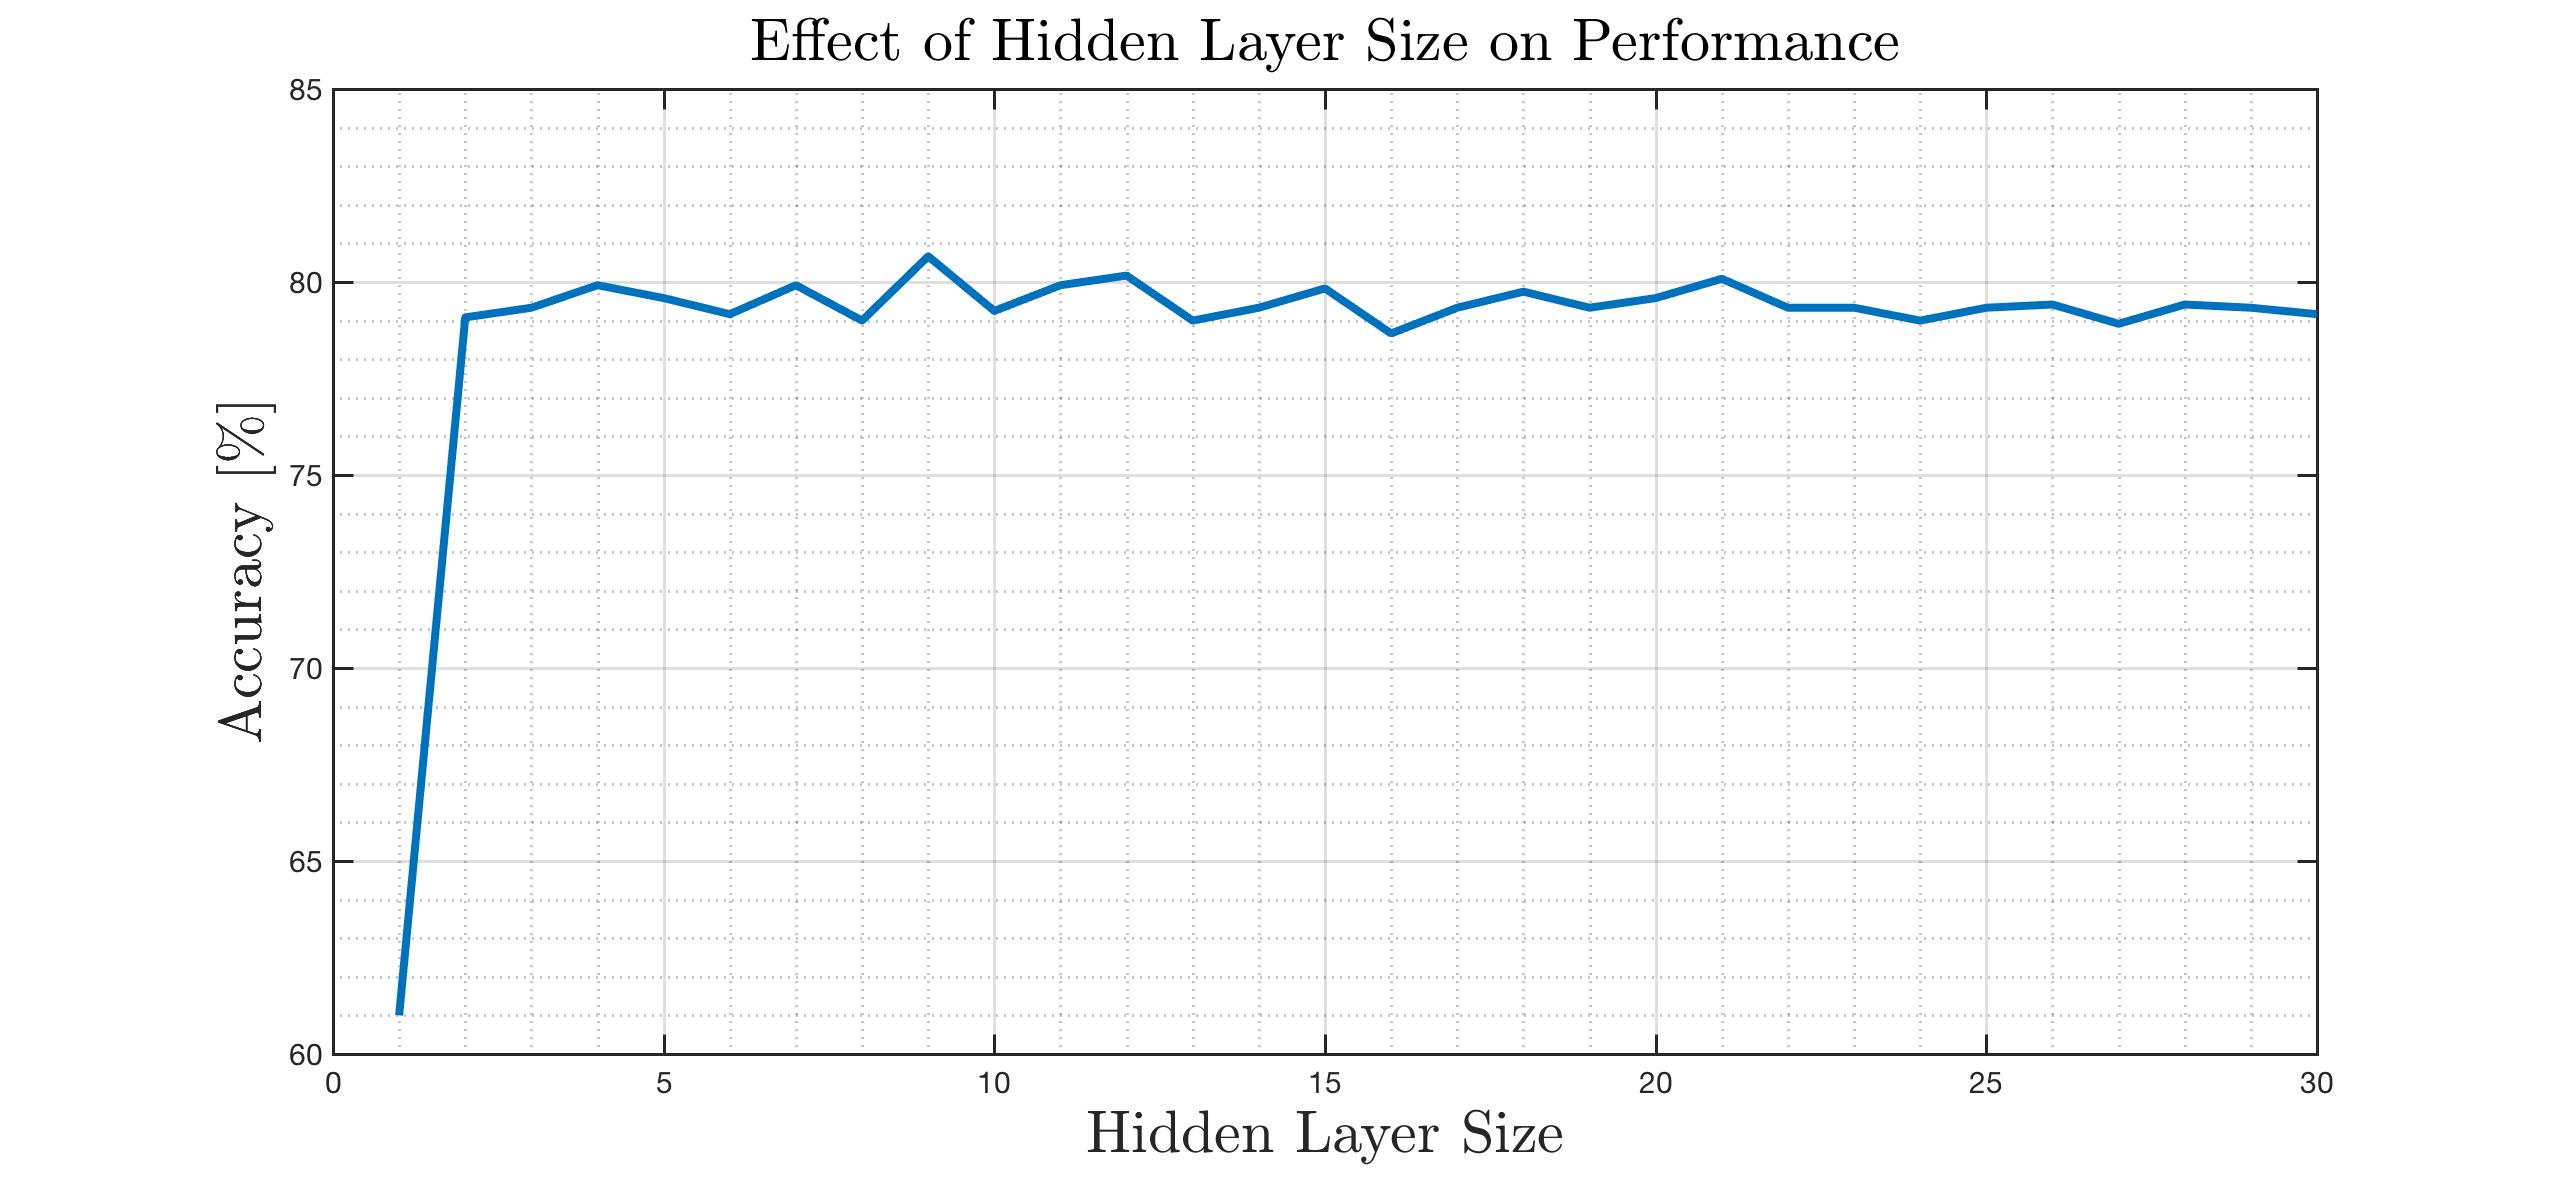
\includegraphics[width=0.45\textwidth]{../results/NN_HiddenLayer}
\caption{Performance vs. Varying Hidden Layer Size
\label{fig:HidSiz}}
\end{figure}

It can be seen that the graph quickly converges to value of roughly 80\% and oscillates around it. In fact it only requires a hidden layer size of 4 to produce hit rate of 79.92\%. When hidden layer is 26, i.e. the recommended starting value, the mean hit rate drops to around 79.46\%. Over the domain from 3 to 30 the accuracy of the Neural Network is relatively constant, deviating by approximately 0.15% from the mean. Thus to maximise time efficiency whilst maintaining accuracy we can use a hidden layer size of 6. We could use 4 or 5, however they are small enough that sometimes they can produce lower hit rates. Size of 6 produces therefore more repeatable results.

\subsection{Number of Hidden Layers}

The optimum number of hidden  layers was then investigated. Source \cite{NN_Java} reports that most problems do not require more than 1 hidden layer, a claim which was also examined.

Having kept the hidden layer size constant at 10, the hidden layer number was varied from 1 to 30, which resulted in the following network being created. Each network was run 7 times and average has been plotted in Figure \ref{fig:HidNum}.

\begin{figure}[H]
\centering
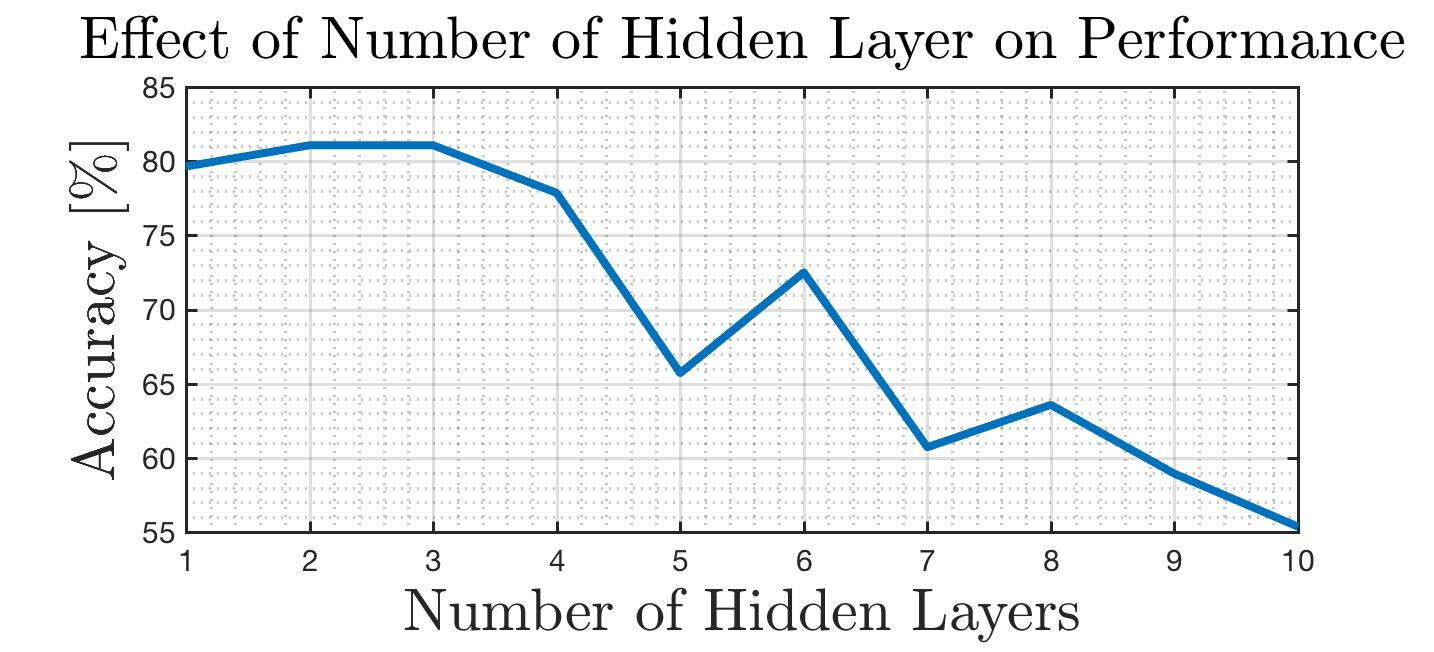
\includegraphics[width=0.45\textwidth]{../results/NN_HiddenLayerNum}
\caption{Performance vs. Varying Number of Hidden Layers
\label{fig:HidNum}}
\end{figure}

We can clearly see that as the number of hidden layers ($numHid$) increases the accuracy drops significantly. Although a peak can be observed at 8 layers, a more reasonable choice would be 3. This is because that the trend after $numHid = 4$ is strictly decreasing until $numHid = 25$. The choice of selecting $numHid = 3$ has also been influenced by the overall time performance of the algorithm.

\subsection{Combined}

Having identified the optimal number of hidden layers and their size independently, we shall investigate how they combine together. In order to achieve that, we have varied both the Size of the Hidden Layers (SHL) and Hidden Layer Number(HLN). Each was varied between 1 and 20. The experiment was repeated three times and mean accuracy was calculated. The resulting graph is shown in Figure \ref{fig:NNSizeNum}.

\begin{figure}
\centering
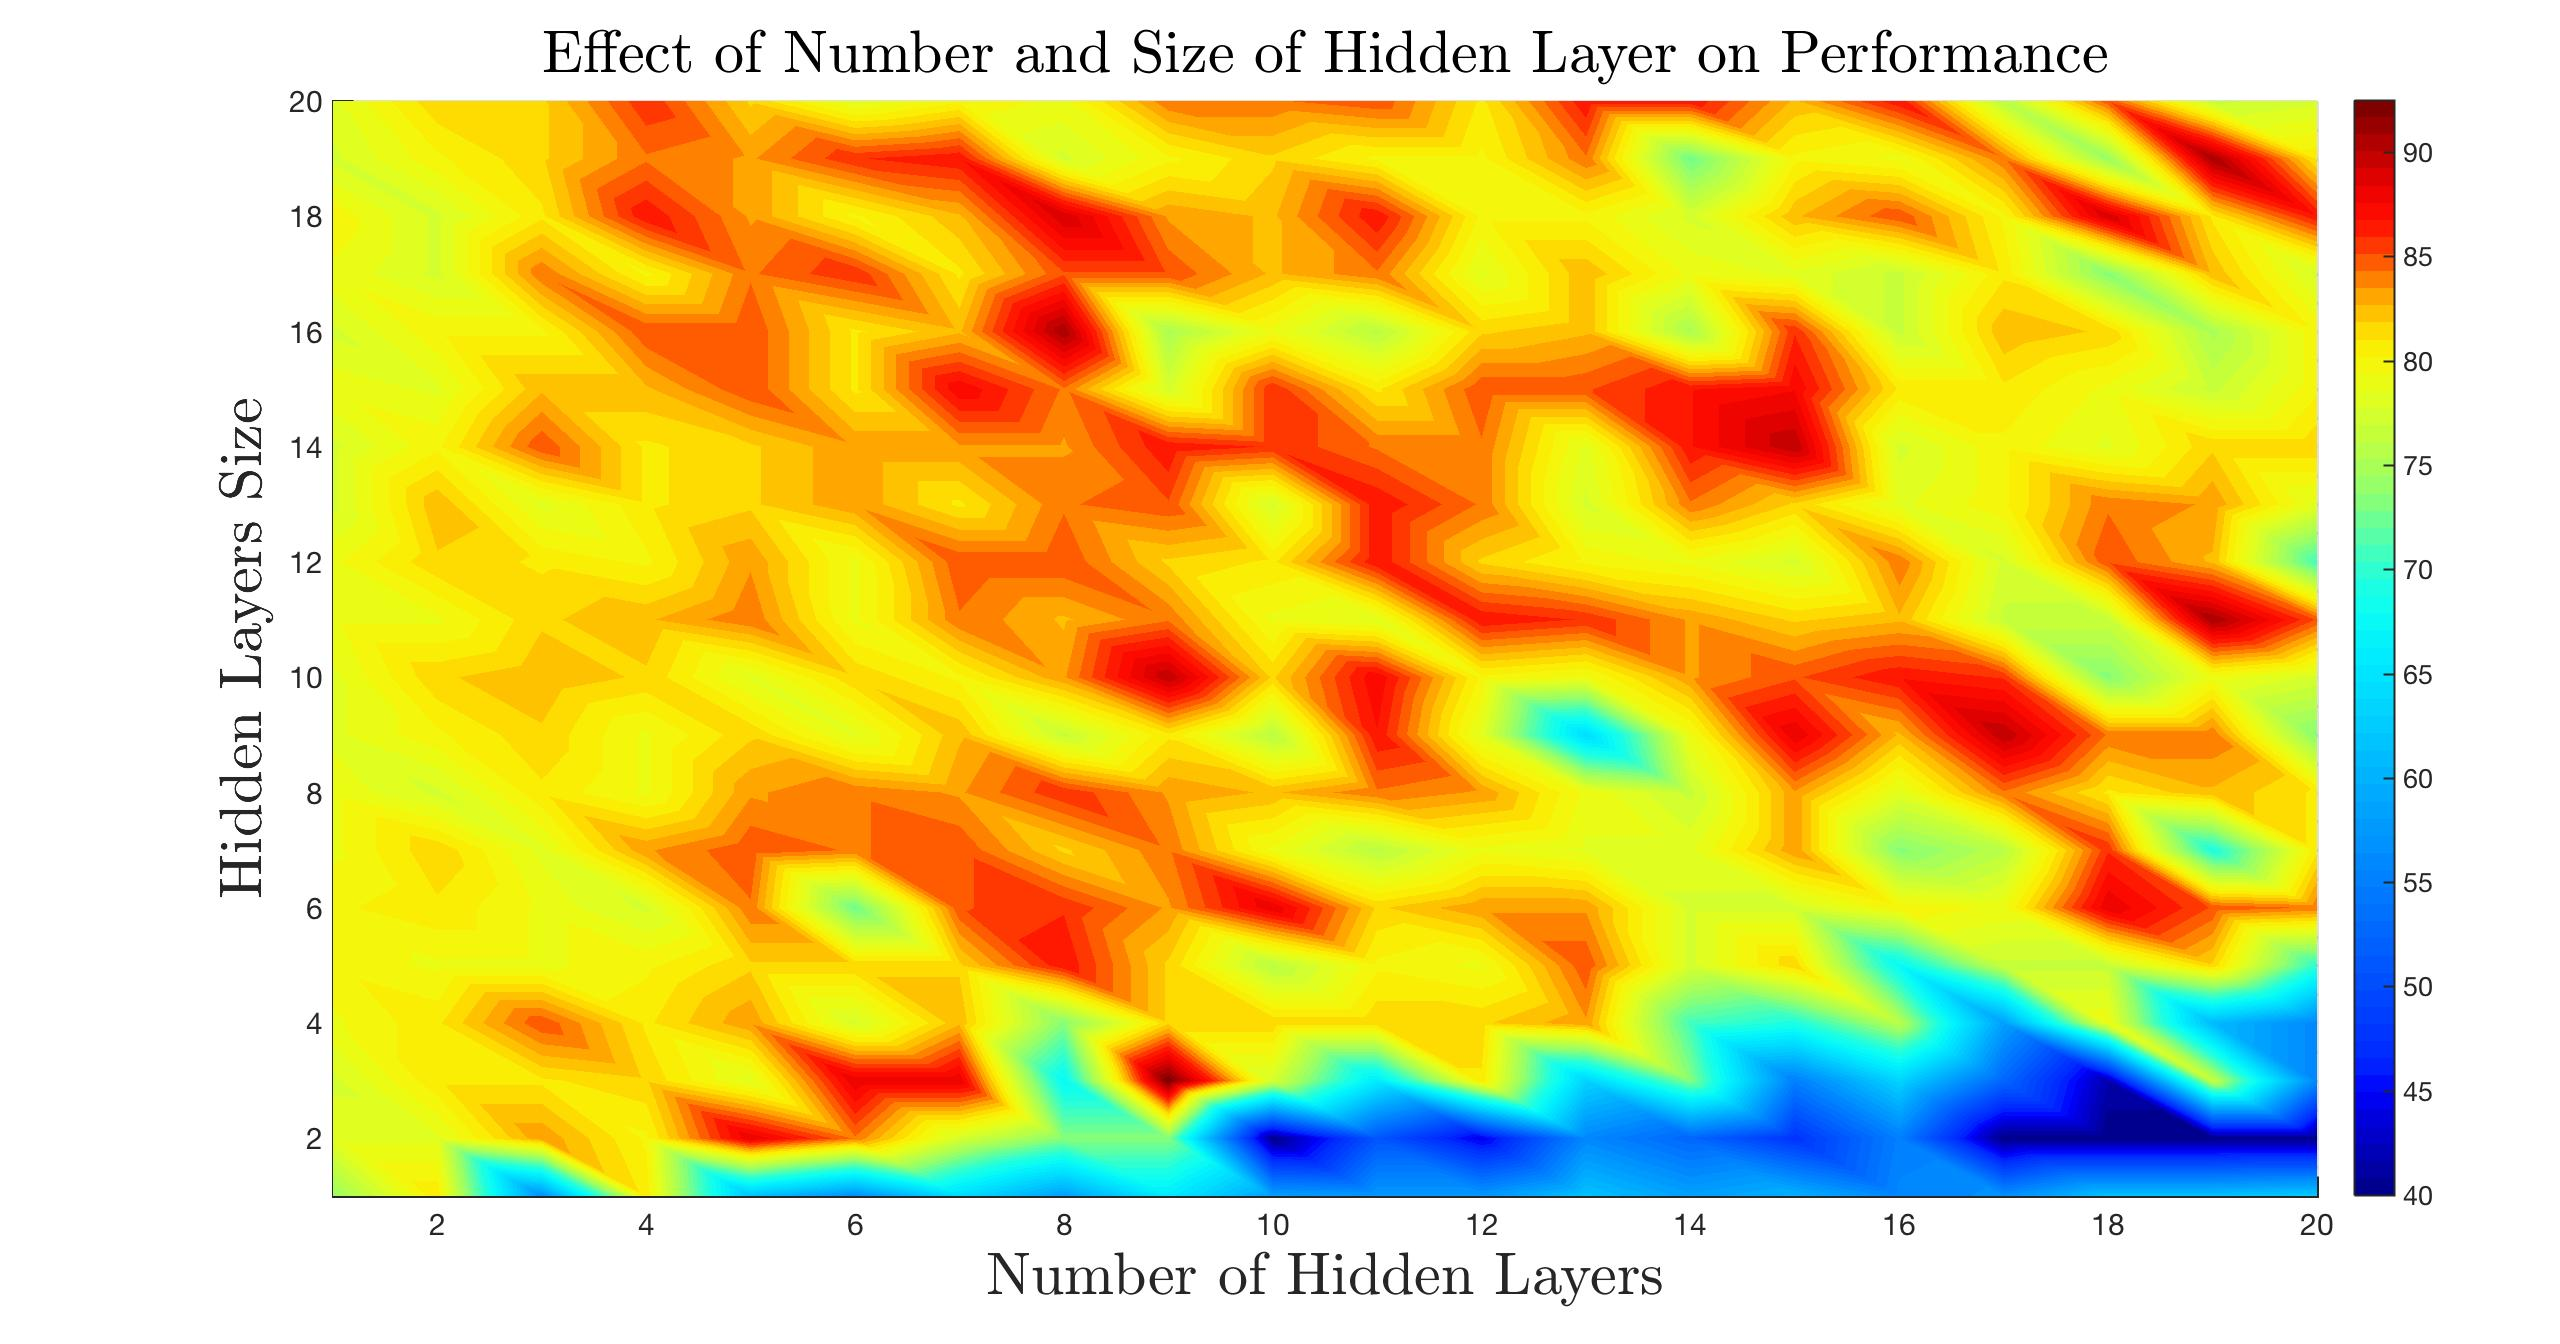
\includegraphics[width=0.45\textwidth]{../results/NN_HidLay_Num_Size4}
\caption{Performance vs. Hidden Layer Number (HLN) vs. Size of Hidden Layer (SHL). Colour scale represents accuracy.
\label{fig:NNSizeNum}}
\end{figure}

We can see a clear skewed line dividing the graph between the red and yellow (accurate) and blue (less accurate) results. Maximum mean accuracy of 92.5\% has been observed for $HLN = 9$ and $SHL = 3$, supporting our earlier observations. However this may be an anomaly, given that the neighbouring region at $HLN = 8$ and $SHL = 3$ produced results of 67.5\%. A clearly more stable region is defined for roughly $SHL > (0.4*HLN-1.2) \quad \forall \quad 20 \geq SHL, HLN \geq 1$, producing high-accuracy, reliable and reproducable results. Hence the best performing combination produces results which on average exceed those obtained using kmeans method by roughly 4 percentage points.

\subsection{Test with Random Data Split}

The data has been split randomly using the Matlab command {\tt\small randperm(178)}. The split ratio has been kept the same as before 118/40/30 (training/testing/validation). The new split has generated much higher accuracy as reported below in Figure \ref{fig:NewSplit}.

\begin{figure}[H]
\centering
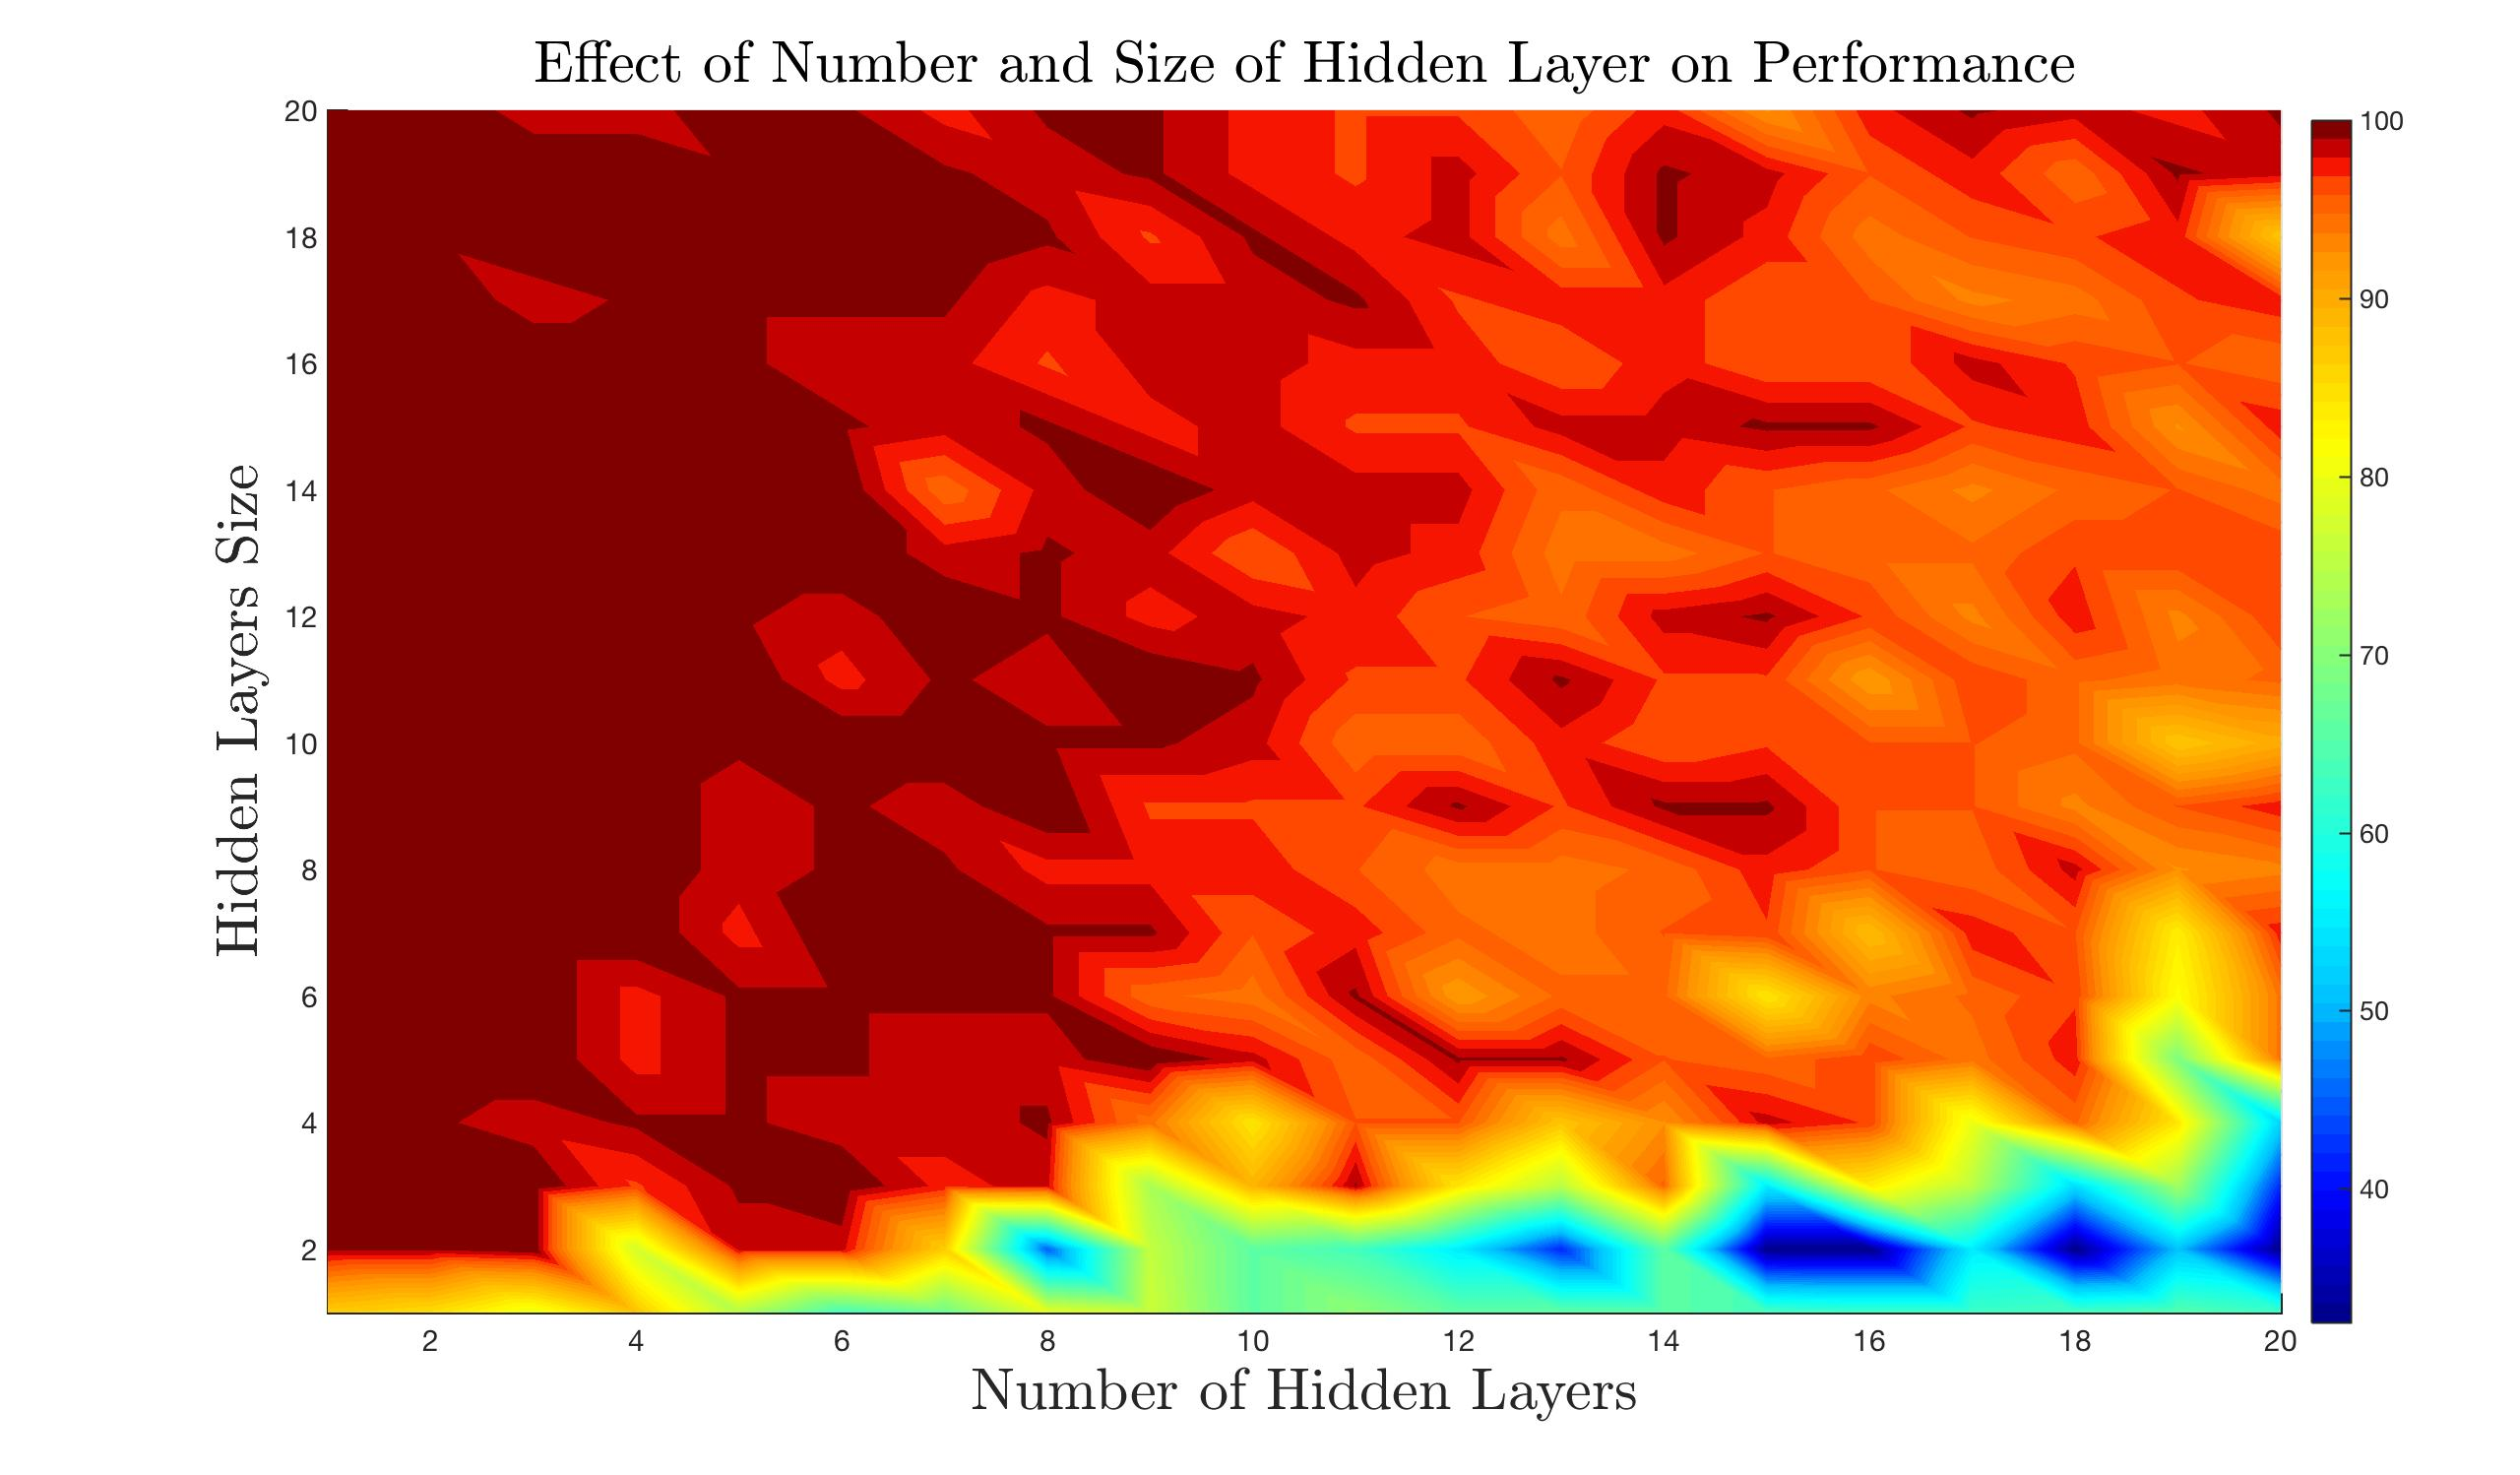
\includegraphics[width=0.45\textwidth]{../results/NN2_2}
\caption{Performance vs. Hidden Layer Number (HLN) vs. Size of Hidden Layer (SHL). Colour represents accuracy rate.
\label{fig:NewSplit}}
\end{figure}
  
Figure \ref{fig:NewSplit} clearly shows that accuracy of 100\% is attainable, demonstrating that the previous data split was unfortunate.

However, in general, the shape of the high accuracy zone is the same as in Figure \ref{fig:NNSizeNum} - $SHL > (0.4*HLN-1.2) \quad \forall \quad 20 \geq SHL, HLN \geq 1$. In this example, we can also identify a region of 100\% accuracy - $SHL > 2 \quad \forall \quad  10 < HLN < 6$ and $10 < SHL$. Therefore taking algorithm execution time into account it would be best to run the neural network with 1 hidden layer and 4 to 6 neurons in it.

\section{Conclusion}

To conclude, L1 clustering was found to be producing the best average results for 3 and 10 means, whereas L2 clustering has been found to be giving maximum accuracy in specific cases. In terms of kNN classification L2, Chi-Square and Mahalanobis distance were almost equally accurate. However in absolute terms, neural networks were found to be most accurate, whilst also being very efficient.

\begin{thebibliography}{9}
\bibitem{wine} 
C. S. Ough\\
\textit{Proline contents of grapes and wines}. \\
Department of Viticulture and Enology, University of California, Davis, USA\\
\url{http://www.vitis-vea.de/admin/volltext/e054492.pdf}

\bibitem{L1L2} 
George Bebis\\
\textit{Advances in Visual Computing, Second International Symposium}.\\
ISVC 2006 Lake Tahoe, NV, USA, November 6-8, 2006. Proceedings, Part II 

\bibitem{MatlabWine}
© The MathWorks, Inc.\\
\textit{Wine Classification}\\
\url{https://uk.mathworks.com/help/nnet/examples/wine-classification.html}

\bibitem{NN_Java}
Jeff Heaton\\
\textit{Programming Neural Networks with Encog3 in Java}\\
Heaton Research, Inc. St. Louis, MO, USA\\
\url{https://s3.amazonaws.com/heatonresearch-books/free/Encog3Java-User.pdf}

\end{thebibliography}

\end{document}
